% -----------------------------------------------------------------------------
\section{Complementary Standards}
\label{sec:complementaryStandards}
% -----------------------------------------------------------------------------
\twoonezero{\subsection{Adding Provenance with PROV-O}
\label{sec:provenance}
\label{sec:wasGeneratedBys}

\vspace{-7pt}
\-\hspace{0.8cm}[New in 2.1.0; see SEP 009: \url{https://github.com/SynBioDex/SEPs/blob/master/sep_009.md}]

Provenance is central to a range of quality control and attribution tasks within the Synthetic Biology design process. Tracking attribution and derivation of one resource from another is paramount for managing intellectual property purposes. Source designs are often modified in systematic ways to generate derived designs, for example, by applying codon optimization or systematically removing all of a class of restriction enzyme sites.  Documenting the transformation used, and any associated parameters, makes this explicit and potentially allows the process to be reproduced systematically. If a design has been used within other designs, and is later found to be defective, it is paramount that all uses of it, including uses of edited versions of the design, can be identified, and ideally replaced with a non-defective alternative. When importing data from external sources, it is important not only to attribute the original source (for example, GenBank), but also the tool used to perform the import, as this may have made arbitrary choices as to how to represent the source knowledge as SBOL. All these activities have in common that it is necessary to track what resource, and what transformation process was applied by whom to derive an SBOL design.

The PROV-O ontology (\url{https://www.w3.org/TR/prov-o/}) already defines a data model for provenance. PROV-O's \sbol{wasDerivedFroms} property was adopted in SBOL 2.x to describe the derivation of an SBOL entity from another in a light-weight provenance scheme.  Here, a subset of PROV-O is adopted for SBOL as a best practice to describe these activities in more detail\footnote{We thank Dr Paolo Missier from the School of Computing Science, Newcastle University for discussions regarding the use of PROV-O.}. PROV-O defines three core classes: \texttt{Entity}, \texttt{Activity} and \texttt{Agent}. An Agent (for example a software or a person) runs an Activity (according to a Plan) to generate one Entity from another. Although, PROV-O provides many other classes and rich set of terms. this specification describes the minimal subset of PROV-O that a provenance-aware SBOL tool should handle. This subset (\ref{uml:provenance}) includes the PROV-O's \sbol{Activity}, \sbol{Usage}, \sbol{Association}, \sbol{Agent} and \sbol{Plan} classes. Any SBOL's \sbol{Identified} object implicitly can act as an instance of PROV-O's \texttt{Entity} class and can include provenance through relationships to different activities. Resources representing \sbol{Agent}, \sbol{Activity} and \sbol{Plan} classes should be handled as \sbol{GenericTopLevel}, whilst \sbol{Usage} and \sbol{Association} resources should be nested within their parent activities. 

%Although the full-set of PROV-O terms can be used in SBOL documents, a subset of PROV-O is adopted as a best practice. It is advised that SBOL tools should at least understand this subset, defined in Figure \ref{uml:provenance}.  

Providers of provenance information are free to make use of more of PROV-O than is described here. It is acceptable for tools that understand more than this subset to use as much as they are able. Tools that only understand this subset must treat any additional data as annotations. Tools that are not aware of SBOL provenance at all must maintain and provide access to this information as annotations. This specification does not state what the newly added properties must point to. As long as they are resources that are consistent with the PROV-O property domains, they are legal. For example, a ComponentDefinition may be derived from another ComponentDefinition, but it would probably not make sense for it to be derived from a Collection.
}

\twotwozero{
The PROV-O specification permits that any kind of SBOL object may be used to generate another. The meaning of these relationships are specified using ontology terms for the \sbolmult{roles:U}{roles} properties on \sbol{Usage} and \sbol{Association} classes.  This specification gives users the flexibility to construct and track provenance histories for their own custom applications, but this flexibility also presents an obstacle to standardized data exchange. Therefore a simple ontology (see \ref{tbl:association_roles} and \ref{tbl:usage_roles}) has been adopted to describe common provenance connections expected in synthetic biology workflows, based on the design-build-test-learn formalization of engineering.

The design-build-test-learn cycle is a common theme in synthetic biology and engineering literature. The design-build-test-learn cycle is the scientific method applied to engineering. Stages of the cycle include designing an initial prototype, testing that prototype, analyzing its performance against specific metrics, learning what worked and what did not work, designing a new prototype based on what was learned, and completing the cycle again. Ideally each iteration of the cycle generates new understanding that feeds back into new cycles as alternative approaches or reformulated problems. Therefore, the design-build-test-learn cycle is a \textit{de facto} ontology upon which to base an SBOL data model for workflow abstraction. Other workflow activities in synthetic biology, such as analyzing, modeling, verifying, and evolving, by and large should fit into this design-build-test-learn abstraction. 

It is expected that users will develop their own ontology terms to specify how SBOL objects are used in a recipe, protocol, or computational analysis. However, these home-made ontologies will be very domain specific, and may not be intelligible to users working in another domain. For example a modeler should not be expected to understand an ontology of \sbol{Usage} \sbolmult{roles:U}{roles} for DNA assembly. The terms ``design'', ``build'', ``test'', and ``learn'' provide a high level workflow abstraction that allows tool-builders to quickly search for and isolate provenance histories relevant to their domain, while keeping track of the flow of data between different users working in different domains of synthetic biology. An example of how these terms are used is provided in \ref{images:design-build-test-learn}.

Provenance semantics defined through \sbol{wasGeneratedBys} relationships are distinctly different from versioning semantics. Generation of a new object is defined by the W3C PROV-O specification as follows:
\begin{quote}
...the completion of production of a new entity by an activity. This entity did not exist before generation and becomes available for usage after this generation.
\end{quote}
These semantics are somewhat different from the versioning semantics defined in section \ref{sec:version}. The SBOL specification defines a new version of an object as an update of a previously published object (and therefore a previously existing object). Therefore, an SBOL object which is ``generated'' from another SHOULD BE regarded as a new entity rather than a new version of an existing entity. However, this distinction is somewhat subjective (see Theseus's paradox). Therefore, we RECOMMEND as a best practice that objects linked by Activities not be successive versions of each other, though this is left to the discretion of users and library developers.
} 

\twotwozero{
\begin{figure}[ht]
\begin{center}
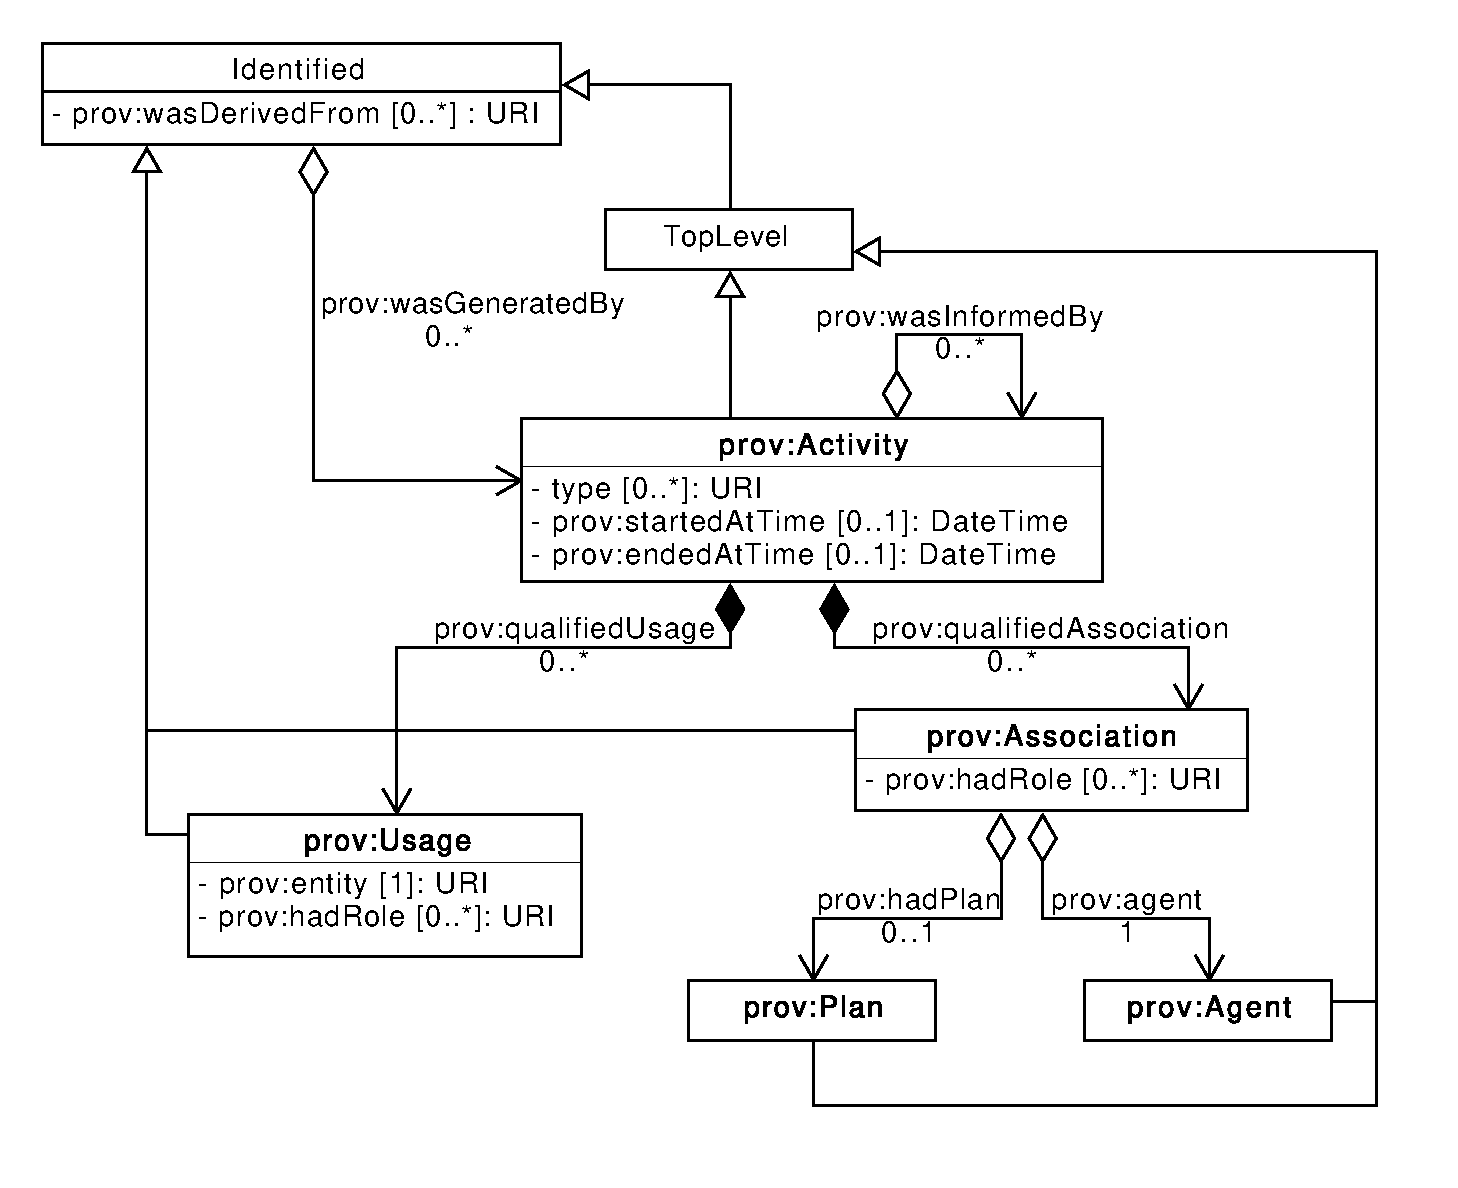
\includegraphics[scale=0.6]{uml/provenance}
\caption[]{Relationships between SBOL and PROV-O classes. The PROV-O classes \external{Activity}, \external{Plan}, and \external{Agent} are all serialized as \sbol{TopLevel} classes in an SBOL document.
\label{uml:provenance}}
\end{center}
\end{figure}
}

\twoonezero{
\subsubsection{Activity}
\label{sec:Activity}

A generated \texttt{Entity} is linked through a \texttt{wasGeneratedBy} relationship to an \sbol{Activity}, which is used to describe how different \sbol{Agent}s and other entities were used. An \sbol{Activity} is linked through a \sbol{associations} to \sbol{Association}s, to describe the role of agents, and is linked through \sbol{usages} to \sbol{Usage}s to describe the role of other entities used as part of the activity. Moreover, each \sbol{Activity} includes optional startedAtTime and endedAtTime properties. When using \sbol{Activity} to capture how an entity was derived, it is expected that any additional information needed will be attached as annotations. This may include software settings or textual notes. Activities can also be linked together using the \sbol{wasInformedBys} relationship to provide dependency without explicitly specifying start and end times.

\paragraph{The \sbolheading{associations} property}\label{sec:associations}
The \sbol{associations} property is OPTIONAL and MAY contain a set of \sbol{URI}s that refers to \sbol{Association} objects.

\paragraph{The \sbolheading{usages} property}\label{sec:usages}
The \sbol{usages} property is OPTIONAL and MAY contain a set of \sbol{URI}s that refers to \sbol{Usage} objects.

\paragraph{The \sbolheading{endedAtTime} property}\label{sec:endedAtTime}
The \sbol{endedAtTime} property is OPTIONAL and contains a DateTime (see section \ref{sec:DateTime}) value, indicating when the activity ended.

\paragraph{The \sbolheading{startedAtTime} property}\label{sec:startedAtTime}
The \sbol{startedAtTime} property is OPTIONAL and contains a DateTime (see section \ref{sec:DateTime}) value, indicating when the activity started.  If this property is present, then the \sbol{endedAtTime} property is REQUIRED.

\paragraph{The \sbolheading{wasInformedBys} property}\label{sec:wasInformedBys}
The \sbol{wasInformedBys} property is OPTIONAL and MAY contain a set of \sbol{URI}s that refers to other \sbol{Activity} objects.

\paragraph{Serialization}
The serialization of an \sbol{Activity} MUST have the following form:
%\twoonezero -end
}

\lstsetsbol
\begin{lstlisting}
<prov:Activity rdf:about="...">
  ... [\emph{properties inherited from identified}] ...
  [\emph{zero or more}]  <prov:qualifiedAssociation>
                   <prov:Association rdf:about="...">...</prov:Association>
                </prov:qualifiedAssociation> [\emph{elements}]
  [\emph{zero or more}]  <prov:qualifiedUsage>
                   <prov:Usage rdf:about="...">...</prov:Usage>
                </prov:qualifiedUsage> [\emph{elements}]             
  [\emph{zero or one}]  <prov:startedAtTime>...</prov:startedAtTime> [\emph{element}]
  [\emph{zero or one}]  <prov:endedAtTime>...</prov:startedAtTime> [\emph{element}] 
  [\emph{zero or more}]  <prov:wasInformedBy rdf:resource="..."/> [\emph{element}] 
</prov:Activity>
\end{lstlisting}

\twotwozero{
Note that the tags prov:qualifiedUsage and prov:qualifiedAssociation are used for \sbol{usages} and \sbol{associations}, respectively.
}

\twoonezero{
\subsubsection{Usage}
\label{sec:Usage}
How different entities are used in an \sbol{Activity} is specified with the \sbol{Usage} class, which is linked from an \sbol{Activity} through the \sbol{Usage} relationship. A \sbol{Usage} is then linked to an \texttt{Entity} through the \texttt{Entity}'s URI and the role of this entity is qualified with the \sbolmult{roles:U}{roles} property. When the \sbol{wasDerivedFroms} property is used together with the full provenance described here, the entity pointed at by the \sbol{wasDerivedFroms} property MUST be included in a \sbol{Usage}.


\paragraph{The \sbolheading{entity} property}\label{sec:entity}
The \sbol{entity} property is REQUIRED and MUST contain a \sbol{URI} which MAY refer to an SBOL Identified object.

\paragraph{The \sbolheading{roles} property}\label{sec:roles:U}
\twotwozero{
The \sbolmult{roles:U}{roles} property is an OPTIONAL set of \sbol{URI}s that refer to particular term(s) describing the usage of an \sbol{entity} referenced by the \sbol{entity} property. Recommended terms that are defined in \ref{tbl:usage_roles} can be used to indicate how the referenced \sbol{entity} is being used in this \sbol{Activity}.
}
}

\twotwozero{
\begin{table}[H]
  \begin{edtable}{tabular}{lp{3.75in}}
    \toprule
    \textbf{URI for Usage roles} & \textbf{Description} \\
    \midrule
    \url{http://sbols.org/v2\#design}	& Design describes the process by which a conceptual representation of an engineer's imagined and intended design for a biological system is derived, possibly from a predictive model or by modifying a pre-existing design. In the context of a \sbol{Usage}, the term indicates that the referenced \sbol{entity} was generated by some previous design \sbol{Activity} and was used by the present \sbol{Activity} as a design for a new object.\\
    \url{http://sbols.org/v2\#build}		& Build describes the process by which a biological construct, sample, or clone is implemented in the laboratory. In the context of a \sbol{Usage}, the term  indicates that the referenced \sbol{entity} was generated by some previous build \sbol{Activity} and was used by the present \sbol{Activity} as a built object.\\
    \url{http://sbols.org/v2\#test}		& Test describes the process of performing experimental measurements to characterize a synthetic biological construct. In the context of a \sbol{Usage}, the term indicates that the referenced \sbol{entity} was generated by some previous test \sbol{Activity} and is used as test data in the present \sbol{Activity}.\\
    \url{http://sbols.org/v2\#learn}	&  Learn describes the process of analyzing experimental measurements to produce a new entity that represents biological knowledge. In the context of a \sbol{Usage}, the term indicates that the referenced \sbol{entity} was generated by some previous learn \sbol{Activity} and is used in the present \sbol{Activity} as a source of scientifically verified knowledge.\\
    \bottomrule
  \end{edtable}
  \caption{Terms to specify the \sbolmult{roles:U}{roles} property of a \sbol{Usage}.}
  \label{tbl:usage_roles}
\end{table}
} 



\twoonezero{
\subsubsection{Association}
\label{sec:Association}
An \sbol{Association} is linked to an \sbol{Agent} through the \sbol{agent} relationship. The \sbol{Association} includes the \sbolmult{roles:A}{roles} property to qualify the role of the \sbol{Agent} in the \sbol{Activity}.

\paragraph{The \sbolheading{agent} property}\label{sec:agent}
The \sbol{agent} property is REQUIRED and MUST contain a \sbol{URI} that refers to an \sbol{Agent} object.

\paragraph{The \sbolheading{roles} property}\label{sec:roles:A}
\twotwozero{ 
The \sbolmult{roles:A}{roles} property is an OPTIONAL set of \sbol{URI}s that refers to particular term(s) that describes the the role of the \sbol{agent} in the parent \sbol{Activity}. 
The recommended terms that are defined in \ref{tbl:association_roles} can be used to specify the kind of \sbol{Activity} performed by the \sbol{Agent}.
}
}

\twothreezero{
\begin{table}[H]
  \begin{edtable}{tabular}{lp{3.75in}}
    \toprule
    \textbf{URI for Association roles} & \textbf{Description} \\
    \midrule
    \url{http://sbols.org/v2\#design}	& Design describes the process by which a conceptual representation of an engineer's imagined and intended design for a biological system is derived, possibly from a predictive model or by modifying a pre-existing design. In the context of an \sbol{Association}, the term design indicates that the \sbol{Agent} performed the parent \sbol{Activity} to generate a design.\\
    \url{http://sbols.org/v2\#build}		& Build describes the process by which a biological construct, sample, or clone is implemented in the laboratory. In the context of an \sbol{Association}, the term build indicates that the \sbol{Agent} performed the parent \sbol{Activity} to implement a design. More generally, the term may represent any kind of experimental manipulation of a biological sample, including propagating, passaging, or evolving cell lines.\\
    \url{http://sbols.org/v2\#test}		& Test describes the process of performing experimental measurements to characterize a synthetic biological construct. In the context of an \sbol{Association}, the \sbol{Agent} performed the parent \sbol{Activity} to perform experimental measurements resulting in raw data represented by an \sbol{ExperimentalData}.\\
    \url{http://sbols.org/v2\#learn}	&  Learn describes the process of analyzing the experimental measurements in order to produce a new entity that represents biological knowledge. In the context of an \sbol{Association}, the \sbol{Agent} processed the raw experimental data to produce an analysis. This process generates a new entity that represents biological knowledge, including tables or graphs referenced by the \sbol{Attachment}s of an \sbol{ExperimentalData}, a \sbol{Model} produced by a fitting process, a consensus \sbol{Sequence} derived from sequencing results, etc.\\
    \bottomrule
  \end{edtable}
  \caption{Terms to specify the \sbolmult{roles:A}{roles} property of an \sbol{Association}.}
  \label{tbl:association_roles}
\end{table}
} 

\twoonezero{
\paragraph{The \sbolheading{plan} property}\label{sec:plan}
The \sbol{plan} property is OPTIONAL and contains a URI that refers to a \sbol{Plan}.

\paragraph{Serialization}
The serialization of an \sbol{Association} MUST have the following form:

} 

\lstsetsbol
\begin{lstlisting}
<prov:Association rdf:about="...">
  ... [\emph{properties inherited from identified}] ...
  [\emph{zero or more}]  <prov:hadRole rdf:resource="..."/> [\emph{element}]
  [\emph{zero or one}]  <prov:hadPlan rdf:resource="..."/> [\emph{element}]
  [\emph{one}]  <prov:agent rdf:resource="..."/> [\emph{element}]
 </prov:Association>
\end{lstlisting}

\twotwozero{
Note that the tags prov:hadRole and prov:hadPlan are used for \sbolmult{roles:A}{roles} and \sbol{plan}, respectively.
}

\subsubsection{Plan}
\label{sec:Plan}
\twoonezero{
 The Plan entity can be used as a place holder to describe the steps (for example scripts or lab protocols) taken when an \sbol{Agent} is used in a particular \sbol{Activity}. 

\paragraph{Serialization}
The serialization of an \sbol{Usage} MUST have the following form:

}%\twoonezero{ end

\lstsetsbol
\begin{lstlisting}
<prov:Plan rdf:about="...">
  ... [\emph{properties inherited from identified}] ...
  ... [\emph{other annotations}] ...
 </prov:Plan>
\end{lstlisting}

\subsubsection{Agent}
\label{sec:Agent}
\twoonezero{
 Examples of agents are person, organization or software. These agents should be annotated with additional information, such as software version, needed to be able to run the same software again.

\paragraph{Serialization}
The serialization of an \sbol{Agent} MUST have the following form:

}%\twoonezero{ end

\lstsetsbol
\begin{lstlisting}
<prov:Agent rdf:about="...">
  ... [\emph{properties inherited from identified}] ...
  ... [\emph{other annotations}] ...
 </prov:Agent>
\end{lstlisting}


\paragraph{Example - Codon optimization}
\twoonezero{
 Codon optimization is a practical real-wold example where provenance properties can be applied. Using the current specification, the relationship between an original CDS and the codon-optimized version could simply be represented using the prov:wasDerivedFrom predicate, in a light-weight form. With more comprehensive use of the PROV ontology, the codon optimization can be represented as an \sbol{Activity}. This \sbol{Activity} can then include additional information, such as the \sbol{Agent} responsible (in this case, codon-optimizing software), and additional parameters.

}%\twoonezero{ end

\lstsetsbol
\begin{lstlisting}
<?xml version="1.0" ?>
<rdf:RDF xmlns:prov="http://www.w3.org/ns/prov#" xmlns:rdf="http://www.w3.org/1999/02/22-rdf-syntax-ns#" xmlns:myapp="http://myapp.com/" xmlns:sbol="http://sbols.org/v2#" xmlns:dcterms="http://purl.org/dc/terms/">
  <sbol:ComponentDefinition rdf:about="http://myapp.com/codon_optimized">
    <sbol:persistentIdentity rdf:resource="http://myapp.com/codon_optimized"/>
    <sbol:displayId>codon_optimized</sbol:displayId>
    <prov:wasDerivedFrom rdf:resource="http://myapp.com/non_codon_optimized"/>
    <prov:wasGeneratedBy rdf:resource="http://myapp.com/codon_optimization_activity"/>
    <dcterms:title>Codon optimized CDS</dcterms:title>
    <sbol:type rdf:resource="http://www.biopax.org/release/biopax-level3.owl#DnaRegion"/>
    <sbol:role rdf:resource="http://identifiers.org/so/SO:0000316"/>
  </sbol:ComponentDefinition>
  <sbol:ComponentDefinition rdf:about="http://myapp.com/non_codon_optimized">
    <sbol:persistentIdentity rdf:resource="http://myapp.com/non_codon_optimized"/>
    <sbol:displayId>non_codon_optimized</sbol:displayId>
    <dcterms:title>Non Codon optimized CDS</dcterms:title>
    <sbol:type rdf:resource="http://www.biopax.org/release/biopax-level3.owl#DnaRegion"/>
    <sbol:role rdf:resource="http://identifiers.org/so/SO:0000316"/>
  </sbol:ComponentDefinition>
  <prov:Activity rdf:about="http://myapp.com/codon_optimization_activity">
    <sbol:persistentIdentity rdf:resource="http://myapp.com/codon_optimization_activity"/>
    <sbol:displayId>codon_optimization_activity</sbol:displayId>
    <dcterms:title>Codon Optimization Activity</dcterms:title>
    <prov:qualifiedAssociation>
      <prov:Association rdf:about="http://myapp.com/codon_optimization_activity/association">
        <sbol:persistentIdentity rdf:resource="http://myapp.com/codon_optimization_activity/association"/>
        <sbol:displayId>association</sbol:displayId>
        <prov:hadRole rdf:resource="http://myapp.com/codonoptimizer"/>
        <prov:agent rdf:resource="http://myapp.com/codon_optimization_software"/>
      </prov:Association>
    </prov:qualifiedAssociation>
    <prov:qualifiedUsage>
      <prov:Usage rdf:about="http://myapp.com/codon_optimization_activity/usage">
        <sbol:persistentIdentity rdf:resource="http://myapp.com/codon_optimization_activity/usage"/>
        <sbol:displayId>usage</sbol:displayId>
        <prov:hadRole rdf:resource="http://sbols.org/v2#source"/>
        <prov:entity rdf:resource="http://myapp.com/non_codon_optimized"/>
      </prov:Usage>
    </prov:qualifiedUsage>
  </prov:Activity>
  <prov:Agent rdf:about="http://myapp.com/codon_optimization_software">
    <sbol:persistentIdentity rdf:resource="http://myapp.com/codon_optimization_software"/>
    <sbol:displayId>codon_optimization_software</sbol:displayId>
    <dcterms:title>Codon Optimization Software</dcterms:title>
  </prov:Agent>
</rdf:RDF>
\end{lstlisting}

\paragraph{Example - Deriving strains}
\twoonezero{
 Bacterial strains are often derived from other strains through modifications such as gene knockouts or mutations. For example, the \texttt{Bacillus subtilis} 168 strain was derived from the NCIMB3610 strain in the 1940s through x-radiation. \textit{B. subtilis} 168 is a laboratory strain and has several advantages as a model organism in synthetic biology. Particularly, the 168 strain is easy to transform and is not motile, facilitating the analysis of engineered cells. The parent strain, on the other hand, is motile but more difficult to transform. The example below shows the derivation of the 168 strain using the new provenance classes.

}%twoonezero end

\lstsetsbol
\begin{lstlisting}
<?xml version="1.0" ?>
<rdf:RDF xmlns:prov="http://www.w3.org/ns/prov#" xmlns:rdf="http://www.w3.org/1999/02/22-rdf-syntax-ns#" xmlns:myapp="http://myapp.com/" xmlns:sbol="http://sbols.org/v2#" xmlns:dcterms="http://purl.org/dc/terms/">
  <sbol:ComponentDefinition rdf:about="http://myapp.com/bsubtilisncimb3610">
    <sbol:persistentIdentity rdf:resource="http://myapp.com/bsubtilisncimb3610"/>
    <sbol:displayId>bsubtilisncimb3610</sbol:displayId>
    <dcterms:title>Bacillus subtilis NCIMB3610</dcterms:title>
    <sbol:type rdf:resource="http://www.biopax.org/release/biopax-level3.owl#DnaRegion"/>
    <sbol:role rdf:resource="http://identifiers.org/so/SO:0000316"/>
  </sbol:ComponentDefinition>
  <sbol:ComponentDefinition rdf:about="http://myapp.com/bsubtilis168">
    <sbol:persistentIdentity rdf:resource="http://myapp.com/bsubtilis168"/>
    <sbol:displayId>bsubtilis168</sbol:displayId>
    <prov:wasDerivedFrom rdf:resource="http://myapp.com/bsubtilisncimb3610"/>
    <prov:wasGeneratedBy rdf:resource="http://myapp.com/xraymutagenesis"/>
    <dcterms:title>Bacillus subtilis 168</dcterms:title>
    <sbol:type rdf:resource="http://www.biopax.org/release/biopax-level3.owl#DnaRegion"/>
    <sbol:role rdf:resource="http://identifiers.org/so/SO:0000316"/>
  </sbol:ComponentDefinition>
  <prov:Activity rdf:about="http://myapp.com/xraymutagenesis">
    <sbol:persistentIdentity rdf:resource="http://myapp.com/xraymutagenesis"/>
    <sbol:displayId>xraymutagenesis</sbol:displayId>
    <dcterms:title>X-ray mutagenesis</dcterms:title>
    <prov:qualifiedAssociation>
      <prov:Association rdf:about="http://myapp.com/xraymutagenesis/association">
        <sbol:persistentIdentity rdf:resource="http://myapp.com/xraymutagenesis/association"/>
        <sbol:displayId>association</sbol:displayId>
        <prov:hadRole rdf:resource="http://myapp.com/mutagen"/>
        <prov:agent rdf:resource="http://myapp.com/x_ray"/>
      </prov:Association>
    </prov:qualifiedAssociation>
    <prov:qualifiedUsage>
      <prov:Usage rdf:about="http://myapp.com/xraymutagenesis/usage">
        <sbol:persistentIdentity rdf:resource="http://myapp.com/xraymutagenesis/usage"/>
        <sbol:displayId>usage</sbol:displayId>
        <prov:hadRole rdf:resource="http://sbols.org/v2#source"/>
        <prov:entity rdf:resource="http://myapp.com/bsubtilisncimb3610"/>
      </prov:Usage>
    </prov:qualifiedUsage>
  </prov:Activity>
  <prov:Agent rdf:about="http://myapp.com/x_ray">
    <sbol:persistentIdentity rdf:resource="http://myapp.com/x_ray"/>
    <sbol:displayId>x_ray</sbol:displayId>
    <dcterms:title>X-ray</dcterms:title>
  </prov:Agent>
</rdf:RDF>
\end{lstlisting}

\paragraph{Example - Design-build-test-learn Workflow}
\twothreezero{
 This particular example represents an idealized workflow for model-based design. The workflow begins with a \sbol{Model} which describes the hypothesized behavior of a biological device. Using a computational tool, a new Design (\sbol{ModuleDefinition}) is composed of biological parts which links back to its \sbol{Model}. A genetic construct is then produced in the laboratory via an assembly protocol, and this biological sample is represented by a Build (\sbol{Implementation}). Once constructed, the Build is then characterized in the laboratory using an automated measurement protocol on a Tecan plate reader, thus generating Test data (represented by an \sbol{ExperimentalData}). Finally, a new \sbol{Model} is derived from these data using some a fitting algorithm implemented in the Python programming language. The final \sbol{Model} may not match the beginning \sbol{Model}, as the observed behavior may not match the prediction. This example illustrates one complete iteration through a design-build-test-learn cycle, as shown in \ref{images:design-build-test-learn}.
}%twotwozero end

\begin{figure}[ht]
\begin{center}
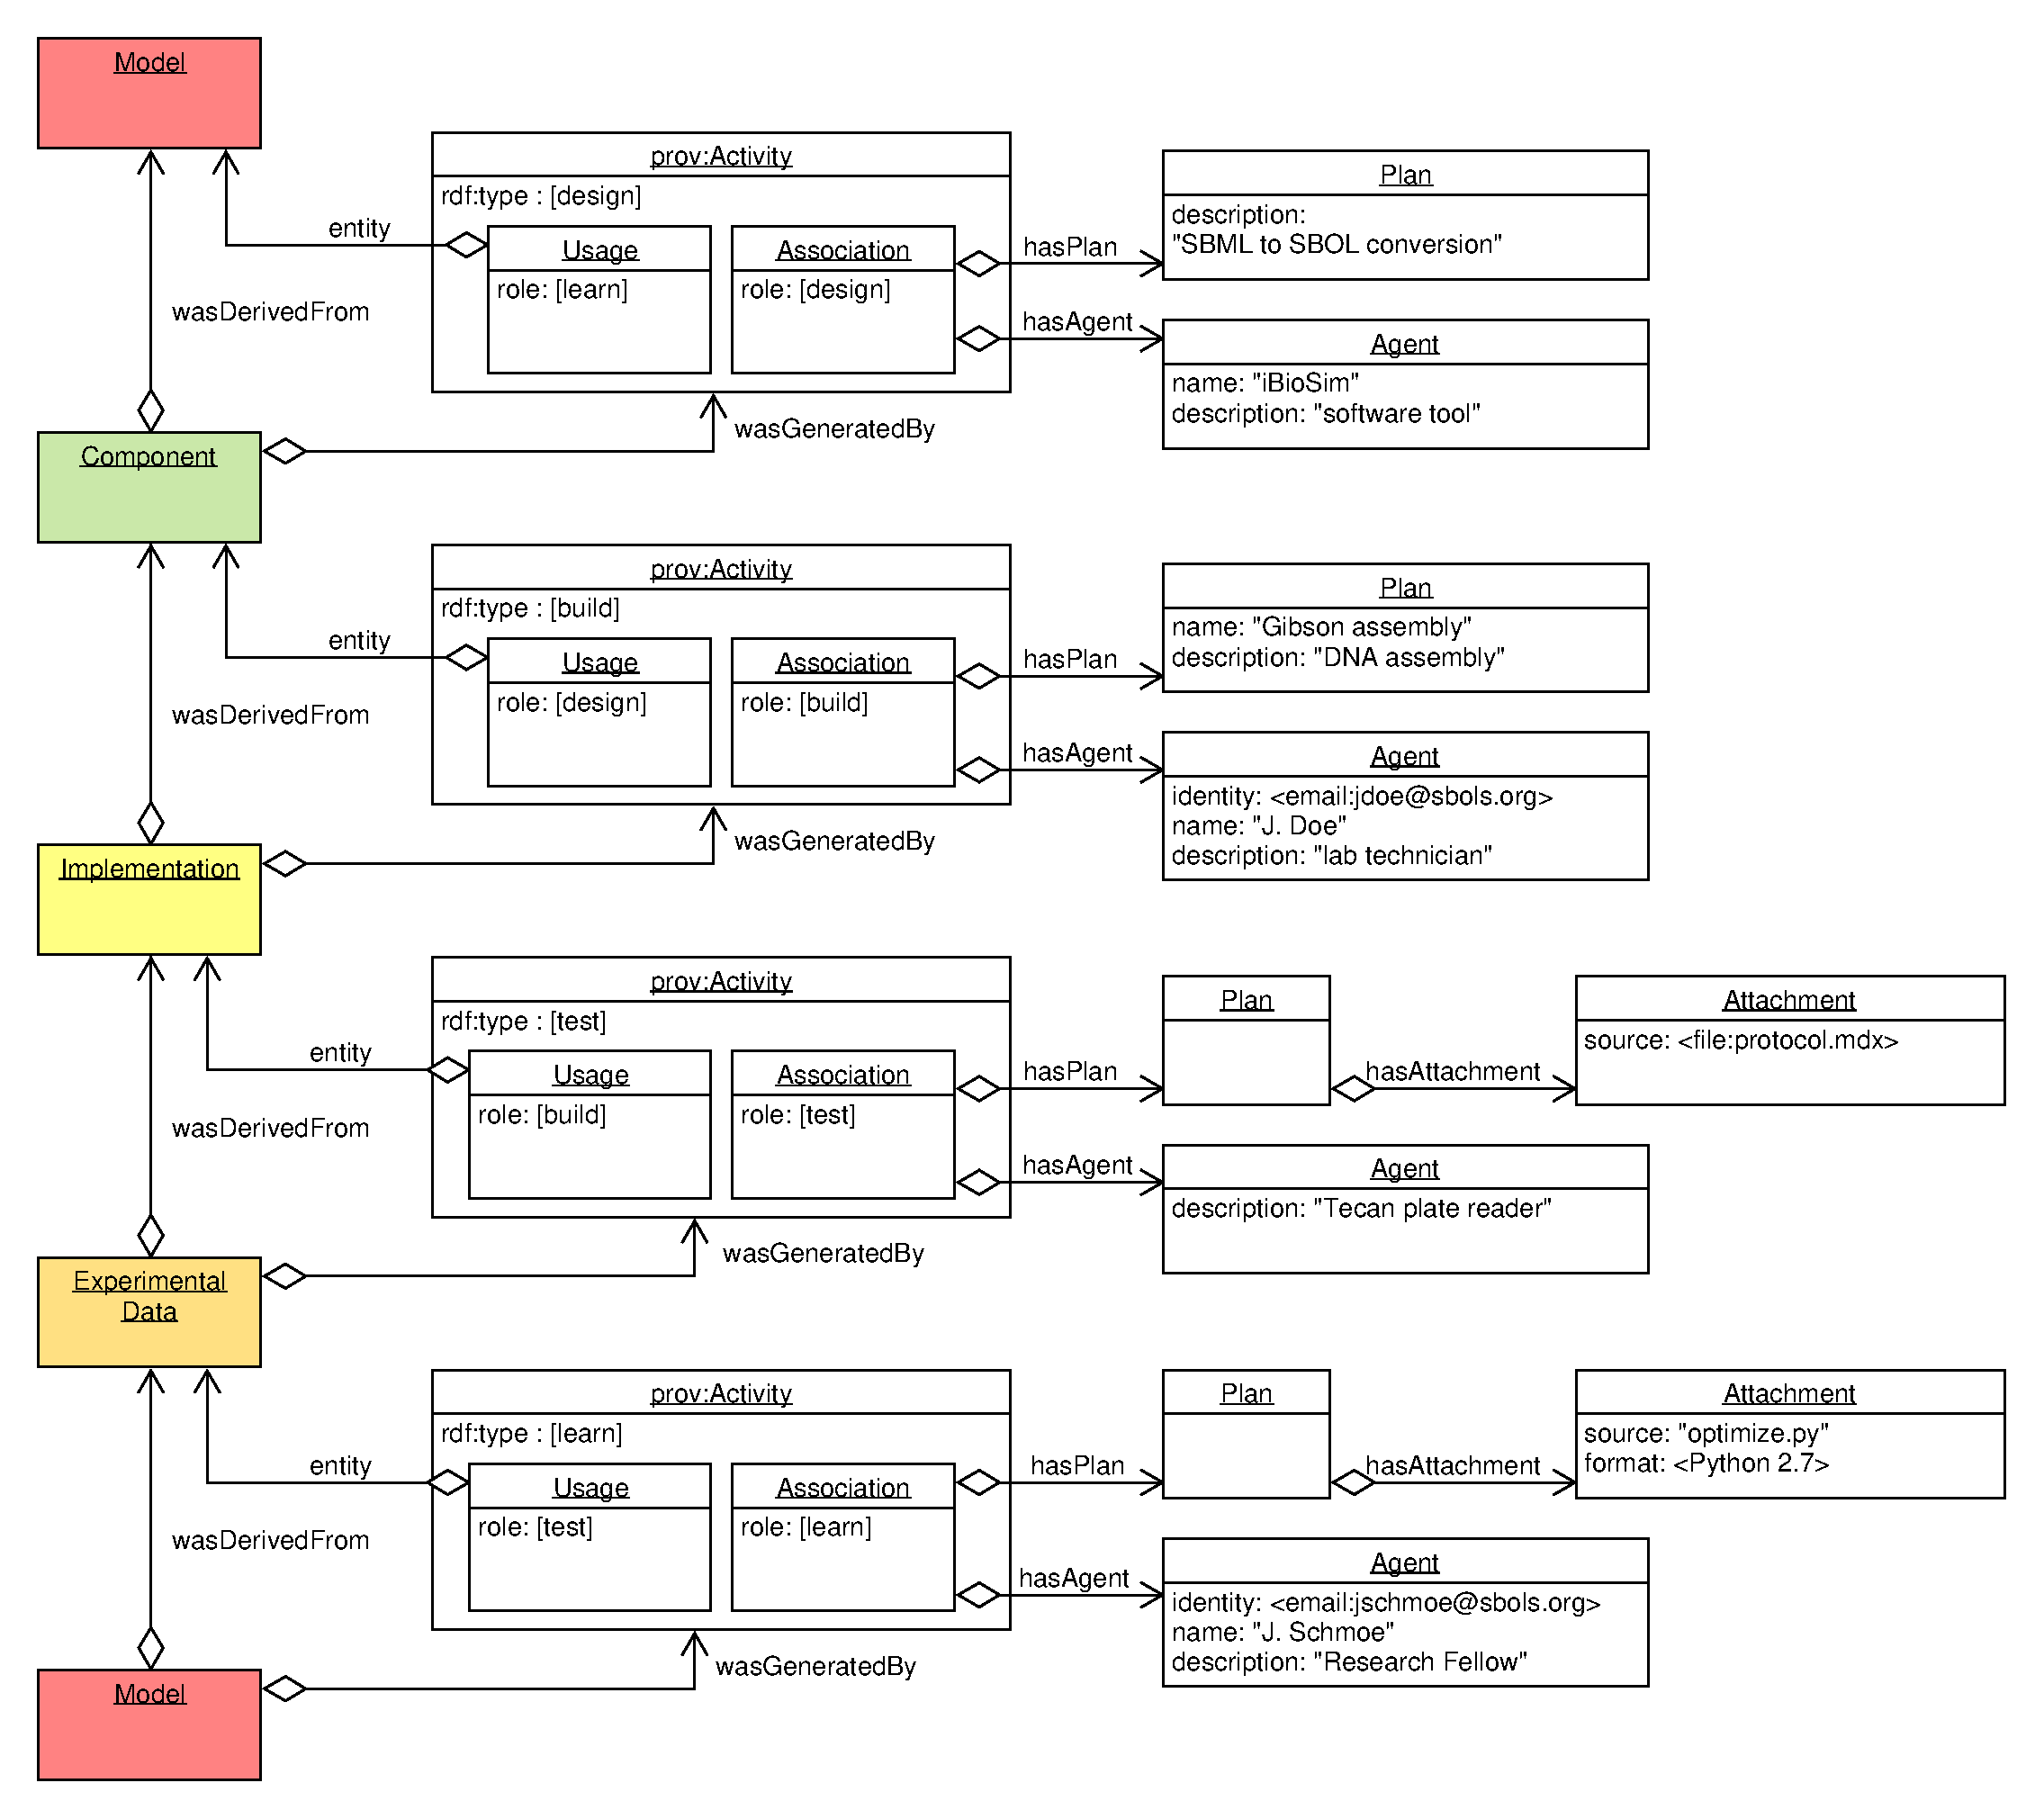
\includegraphics[width=\linewidth]{uml/design-build-test}
\caption[]{An example data structure representing an idealized workflow for model-based
design}
\label{images:design-build-test-learn}
\end{center}
\end{figure}

%% proposed by issue #137
\clearpage

\twotwoone{}
\lstsetsbol
\begin{lstlisting}
<?xml version="1.0" encoding="utf-8"?>
<rdf:RDF xmlns:dcterms="http://purl.org/dc/terms/" xmlns:prov="http://www.w3.org/ns/prov#" xmlns:rdf="http://www.w3.org/1999/02/22-rdf-syntax-ns#" xmlns:sbol="http://sbols.org/v2#" xmlns:sys-bio="http://sys-bio.org#">
  <prov:Activity rdf:about="http://sys-bio.org/Activity_build_generation/1.0.0">
    <sbol:displayId>Activity_build_generation</sbol:displayId>
    <sbol:persistentIdentity rdf:resource="http://sys-bio.org/Activity_build_generation"/>
    <sbol:version>1.0.0</sbol:version>
    <prov:qualifiedAssociation>
      <prov:Association rdf:about="http://sys-bio.org/Activity_build_generation/build_generation_association/1.0.0">
        <sbol:displayId>build_generation_association</sbol:displayId>
        <sbol:persistentIdentity rdf:resource="http://sys-bio.org/Activity_build_generation/build_generation_association"/>
        <sbol:version>1.0.0</sbol:version>
        <prov:agent rdf:resource="https://synbiohub.org/jdoe/1.0.0"/>
        <prov:hadPlan rdf:resource="http://sys-bio.org/Plan_gibson_assembly/1.0.0"/>
        <prov:hadRole rdf:resource="http://sbols.org/v2#build"/>
      </prov:Association>
    </prov:qualifiedAssociation>
    <prov:qualifiedUsage>
      <prov:Usage rdf:about="http://sys-bio.org/Activity_build_generation/design_usage/1.0.0">
        <sbol:displayId>design_usage</sbol:displayId>
        <sbol:persistentIdentity rdf:resource="http://sys-bio.org/Activity_build_generation/design_usage"/>
        <sbol:version>1.0.0</sbol:version>
        <prov:entity rdf:resource="http://sys-bio.org/ModuleDefinition_design/1.0.0"/>
        <prov:hadRole rdf:resource="http://sbols.org/v2#design"/>
      </prov:Usage>
    </prov:qualifiedUsage>
  </prov:Activity>
  <prov:Activity rdf:about="http://sys-bio.org/Activity_design_generation/1.0.0">
    <sbol:displayId>Activity_design_generation</sbol:displayId>
    <sbol:persistentIdentity rdf:resource="http://sys-bio.org/Activity_design_generation"/>
    <sbol:version>1.0.0</sbol:version>
    <prov:qualifiedAssociation>
      <prov:Association rdf:about="http://sys-bio.org/Activity_design_generation/design_generation_association/1.0.0">
        <sbol:displayId>design_generation_association</sbol:displayId>
        <sbol:persistentIdentity rdf:resource="http://sys-bio.org/Activity_design_generation/design_generation_association"/>
        <sbol:version>1.0.0</sbol:version>
        <prov:agent rdf:resource="http://www.async.ece.utah.edu/ibiosim"/>
        <prov:hadPlan rdf:resource="http://sys-bio.org/Plan_conversion/1.0.0"/>
        <prov:hadRole rdf:resource="http://sbols.org/v2#design"/>
      </prov:Association>
    </prov:qualifiedAssociation>
    <prov:qualifiedUsage>
      <prov:Usage rdf:about="http://sys-bio.org/Activity_design_generation/predicted_usage/1.0.0">
        <sbol:displayId>predicted_usage</sbol:displayId>
        <sbol:persistentIdentity rdf:resource="http://sys-bio.org/Activity_design_generation/predicted_usage"/>
        <sbol:version>1.0.0</sbol:version>
        <prov:entity rdf:resource="http://sys-bio.org/Model_predicted/1.0.0"/>
        <prov:hadRole rdf:resource="http://sbols.org/v2#learn"/>
      </prov:Usage>
    </prov:qualifiedUsage>
  </prov:Activity>
  <prov:Activity rdf:about="http://sys-bio.org/Activity_fit_model_generation/1.0.0">
    <sbol:displayId>Activity_fit_model_generation</sbol:displayId>
    <sbol:persistentIdentity rdf:resource="http://sys-bio.org/Activity_fit_model_generation"/>
    <sbol:version>1.0.0</sbol:version>
    <prov:qualifiedAssociation>
      <prov:Association rdf:about="http://sys-bio.org/Activity_fit_model_generation/fit_model_generation_association/1.0.0">
        <sbol:displayId>fit_model_generation_association</sbol:displayId>
        <sbol:persistentIdentity rdf:resource="http://sys-bio.org/Activity_fit_model_generation/fit_model_generation_association"/>
        <sbol:version>1.0.0</sbol:version>
        <prov:agent rdf:resource="https://synbiohub.org/jschmoe/1.0.0"/>
        <prov:hadPlan rdf:resource="http://sys-bio.org/Plan_model_fitting/1.0.0"/>
        <prov:hadRole rdf:resource="http://sbols.org/v2#learn"/>
      </prov:Association>
    </prov:qualifiedAssociation>
    <prov:qualifiedUsage>
      <prov:Usage rdf:about="http://sys-bio.org/Activity_fit_model_generation/raw_data_usage/1.0.0">
        <sbol:displayId>raw_data_usage</sbol:displayId>
        <sbol:persistentIdentity rdf:resource="http://sys-bio.org/Activity_fit_model_generation/raw_data_usage"/>
        <sbol:version>1.0.0</sbol:version>
        <prov:entity rdf:resource="http://sys-bio.org/ExperimentalData_raw_data/1.0.0"/>
        <prov:hadRole rdf:resource="http://sbols.org/v2#test"/>
      </prov:Usage>
    </prov:qualifiedUsage>
  </prov:Activity>
  <prov:Activity rdf:about="http://sys-bio.org/Activity_raw_data_generation/1.0.0">
    <sbol:displayId>Activity_raw_data_generation</sbol:displayId>
    <sbol:persistentIdentity rdf:resource="http://sys-bio.org/Activity_raw_data_generation"/>
    <sbol:version>1.0.0</sbol:version>
    <prov:qualifiedAssociation>
      <prov:Association rdf:about="http://sys-bio.org/Activity_raw_data_generation/raw_data_generation_association/1.0.0">
        <sbol:displayId>raw_data_generation_association</sbol:displayId>
        <sbol:persistentIdentity rdf:resource="http://sys-bio.org/Activity_raw_data_generation/raw_data_generation_association"/>
        <sbol:version>1.0.0</sbol:version>
        <prov:agent rdf:resource="http://sys-bio.org/plate_reader_1"/>
        <prov:hadPlan rdf:resource="http://sys-bio.org/Plan_characterization_protocol/1.0.0"/>
        <prov:hadRole rdf:resource="http://sbols.org/v2#test"/>
      </prov:Association>
    </prov:qualifiedAssociation>
    <prov:qualifiedUsage>
      <prov:Usage rdf:about="http://sys-bio.org/Activity_raw_data_generation/build_usage/1.0.0">
        <sbol:displayId>build_usage</sbol:displayId>
        <sbol:persistentIdentity rdf:resource="http://sys-bio.org/Activity_raw_data_generation/build_usage"/>
        <sbol:version>1.0.0</sbol:version>
        <prov:entity rdf:resource="http://sys-bio.org/Implementation_build/1.0.0"/>
        <prov:hadRole rdf:resource="http://sbols.org/v2#build"/>
      </prov:Usage>
    </prov:qualifiedUsage>
  </prov:Activity>
  <sbol:Attachment rdf:about="http://sys-bio.org/Attachment_characterization_protocol/1.0.0">
    <sbol:displayId>Attachment_characterization_protocol</sbol:displayId>
    <sbol:persistentIdentity rdf:resource="http://sys-bio.org/Attachment_characterization_protocol"/>
    <sbol:source rdf:resource="dynamic_measurement.mdx"/>
    <sbol:version>1.0.0</sbol:version>
  </sbol:Attachment>
  <sbol:Attachment rdf:about="http://sys-bio.org/Attachment_model_fitting_script/1.0.0">
    <sbol:displayId>Attachment_model_fitting_script</sbol:displayId>
    <sbol:format rdf:resource="http://www.ebi.ac.uk/swo/SWO_0000147"></sbol:format>
    <sbol:persistentIdentity rdf:resource="http://sys-bio.org/Attachment_model_fitting_script"/>
    <sbol:source rdf:resource="file://server.sys-bio.org/Dev/optimize.py"/>
    <sbol:version>1.0.0</sbol:version>
  </sbol:Attachment>
  <sbol:ExperimentalData rdf:about="http://sys-bio.org/ExperimentalData_raw_data/1.0.0">
    <sbol:displayId>ExperimentalData_raw_data</sbol:displayId>
    <sbol:persistentIdentity rdf:resource="http://sys-bio.org/ExperimentalData_raw_data"/>
    <sbol:attachment rdf:resource="http://sys-bio.org/Attachment_raw_data/1.0.0"/>
    <sbol:version>1.0.0</sbol:version>
    <prov:wasDerivedFrom rdf:resource="http://sys-bio.org/Implementation_build/1.0.0"/>
    <prov:wasGeneratedBy rdf:resource="http://sys-bio.org/Activity_raw_data_generation/1.0.0"/>
  </sbol:ExperimentalData>
  <sbol:Attachment rdf:about="http://sys-bio.org/Attachment_raw_data/1.0.0">
    <sbol:displayId>Attachment_raw_data</sbol:displayId>
    <sbol:format rdf:resource="http://edamontology.org/format_3752"/>
    <sbol:persistentIdentity rdf:resource="http://sys-bio.org/Attachment_raw_data"/>
    <sbol:source rdf:resource="file://server.sys-bio.org/data/plate_reader_expt_012218.csv"/>
    <sbol:version>1.0.0</sbol:version>
  </sbol:Attachment>
  <sbol:Implementation rdf:about="http://sys-bio.org/Implementation_build/1.0.0">
    <sbol:displayId>Implementation_build</sbol:displayId>
    <sbol:persistentIdentity rdf:resource="http://sys-bio.org/Implementation_build"/>
    <sbol:version>1.0.0</sbol:version>
    <prov:wasDerivedFrom rdf:resource="http://sys-bio.org/ModuleDefinition_design/1.0.0"/>
    <prov:wasGeneratedBy rdf:resource="http://sys-bio.org/Activity_build_generation/1.0.0"/>
  </sbol:Implementation>
  <sbol:Model rdf:about="http://sys-bio.org/Model_fit_model/1.0.0">
    <sbol:displayId>Model_fit_model</sbol:displayId>
    <sbol:framework rdf:resource="http://identifiers.org/biomodels.sbo/SBO:0000062"/>
    <sbol:language rdf:resource="http://identifiers.org/edam/format_2585"/>
    <sbol:persistentIdentity rdf:resource="http://sys-bio.org/Model_fit_model"/>
    <sbol:source rdf:resource="file://server.sys-bio.org/models/model_fit.xml"/>
    <sbol:version>1.0.0</sbol:version>
    <prov:wasDerivedFrom rdf:resource="http://sys-bio.org/ExperimentalData_raw_data/1.0.0"/>
    <prov:wasGeneratedBy rdf:resource="http://sys-bio.org/Activity_fit_model_generation/1.0.0"/>
  </sbol:Model>
  <sbol:Model rdf:about="http://sys-bio.org/Model_predicted/1.0.0">
    <sbol:displayId>Model_predicted</sbol:displayId>
    <sbol:framework rdf:resource="http://identifiers.org/biomodels.sbo/SBO:0000062"/>
    <sbol:language rdf:resource="http://identifiers.org/edam/format_2585"/>
    <sbol:persistentIdentity rdf:resource="http://sys-bio.org/Model_predicted"/>
    <sbol:source rdf:resource="file://server.sys-bio.org/circuit_simulation.xml"/>
    <sbol:version>1.0.0</sbol:version>
  </sbol:Model>
  <sbol:ModuleDefinition rdf:about="http://sys-bio.org/ModuleDefinition_design/1.0.0">
    <sbol:displayId>ModuleDefinition_design</sbol:displayId>
    <sbol:persistentIdentity rdf:resource="http://sys-bio.org/ModuleDefinition_design"/>
    <sbol:version>1.0.0</sbol:version>
    <prov:wasDerivedFrom rdf:resource="http://sys-bio.org/Model_predicted/1.0.0"/>
    <prov:wasGeneratedBy rdf:resource="http://sys-bio.org/Activity_design_generation/1.0.0"/>
  </sbol:ModuleDefinition>
  <prov:Plan rdf:about="http://sys-bio.org/Plan_characterization_protocol/1.0.0">
    <sbol:attachment rdf:resource="http://sys-bio.org/Attachment_characterization_protocol/1.0.0"/>
    <sbol:displayId>Plan_characterization_protocol</sbol:displayId>
    <sbol:persistentIdentity rdf:resource="http://sys-bio.org/Plan_characterization_protocol"/>
    <sbol:version>1.0.0</sbol:version>
  </prov:Plan>
  <prov:Plan rdf:about="http://sys-bio.org/Plan_conversion/1.0.0">
    <dcterms:description>SBML to SBOL conversion</dcterms:description>
    <sbol:displayId>Plan_conversion</sbol:displayId>
    <sbol:persistentIdentity rdf:resource="http://sys-bio.org/Plan_conversion"/>
    <sbol:version>1.0.0</sbol:version>
  </prov:Plan>
  <prov:Plan rdf:about="http://sys-bio.org/Plan_gibson_assembly/1.0.0">
    <dcterms:description>DNA assembly</dcterms:description>
    <sbol:displayId>Plan_gibson_assembly</sbol:displayId>
    <sbol:persistentIdentity rdf:resource="http://sys-bio.org/Plan_gibson_assembly"/>
    <sbol:version>1.0.0</sbol:version>
  </prov:Plan>
  <prov:Plan rdf:about="http://sys-bio.org/Plan_model_fitting/1.0.0">
    <sbol:attachment rdf:resource="http://sys-bio.org/Attachment_model_fitting_script/1.0.0"/>
    <sbol:displayId>Plan_model_fitting</sbol:displayId>
    <sbol:persistentIdentity rdf:resource="http://sys-bio.org/Plan_model_fitting"/>
    <sbol:version>1.0.0</sbol:version>
  </prov:Plan>
  <prov:Agent rdf:about="http://sys-bio.org/plate_reader_1/1.0.0">
    <sbol:persistentIdentity rdf:resource="http://sys-bio.org/plate_reader_1"></sbol:persistentIdentity>
    <sbol:version>1.0.0</sbol:version>
    <sbol:displayId>plate_reader_1</sbol:displayId>
  </prov:Agent>
  <prov:Agent rdf:about="http://www.async.ece.utah.edu/ibiosim/1.0.0">
    <dcterms:description>Software application for the modeling, analysis, and design of genetic circuits</dcterms:description>
    <sbol:persistentIdentity rdf:resource="http://www.async.ece.utah.edu/ibiosim"/>
    <sbol:version>1.0.0</sbol:version>
    <sbol:displayId>ibiosim</sbol:displayId>
  </prov:Agent>
  <prov:Agent rdf:about="https://synbiohub.org/jdoe/1.0.0">
    <dcterms:description>Lab Technician</dcterms:description>
    <dcterms:title>John Doe</dcterms:title>
    <sbol:persistentIdentity rdf:resource="https://synbiohub.org/jdoe"/>
    <sbol:version>1.0.0</sbol:version>
    <sbol:displayId>jdoe</sbol:displayId>
  </prov:Agent>
  <prov:Agent rdf:about="https://synbiohub.org/jschmoe/1.0.0">
    <dcterms:description>Research Fellow</dcterms:description>
    <dcterms:title>Joe Schmoe</dcterms:title>
    <sbol:persistentIdentity rdf:resource="https://synbiohub.org/jschmoe"/>
    <sbol:version>1.0.0</sbol:version>
    <sbol:displayId>jschmoe</sbol:displayId>
  </prov:Agent>
</rdf:RDF>
\end{lstlisting}

\twotwoone{
  \paragraph{Example - Combinatorial Derivation}
  This example illustrates how the Prov ontology should be used to reference to link a generated design to the combinatorial derivation that it was generated from.  In this example, there is a top-level derivation (Promoter\_Derivation) which specifies two possible promoters for this design, as well as an additional derivation (Terminator\_Derivation) to be used for the Gen\_Component.  The second derivation (Terminator\_Derivation) specifies two possible terminators to used within the Gen\_Component.  The derived design (Derivation\_example\_GeneratedInstance11) has a reference in the \sbol{wasDerivedFroms} list to the \sbol{CombinatorialDerivation} that it was derived from (i.e., Promoter\_Derivation).  Also, each component has reference in the \sbol{wasDerivedFroms} list to the component within the \sbol{template} that it is derived from.  The Gen\_Component in this derived design refers to a derived design for it (i.e., Gen\_GeneratedInstance1).  This design has a reference in the \sbol{wasDerivedFroms} list that refers to the \sbol{CombinatorialDerivation} that is used to derive it (i.e., Terminator\_Derivation).  Once again, each component has a reference in the \sbol{wasDerivedFroms} list to the component within the \sbol{template} that it is derived from.  The advantage of these provenance links is that they provide sufficient information to validate that this derived design has been properly derived from the specified \sbol{CombinatorialDerivation}s.
}

\begin{lstlisting}
<?xml version="1.0" ?>
<rdf:RDF xmlns:rdf="http://www.w3.org/1999/02/22-rdf-syntax-ns#" xmlns:sbh="http://wiki.synbiohub.org/wiki/Terms/synbiohub#" xmlns:sbol="http://sbols.org/v2#" xmlns:dcterms="http://purl.org/dc/terms/" xmlns:prov="http://www.w3.org/ns/prov#" xmlns:dc="http://purl.org/dc/elements/1.1/">
  <sbol:ComponentDefinition rdf:about="https://synbiohub.programmingbiology.org/public/Cello_Parts/P1/1">
    <sbol:persistentIdentity rdf:resource="https://synbiohub.programmingbiology.org/public/Cello_Parts/P1"/>
    <sbol:displayId>P1</sbol:displayId>
    <sbol:version>1</sbol:version>
    <prov:wasGeneratedBy rdf:resource="https://synbiohub.programmingbiology.org/public/Cello_Parts/CelloUCF2sbol_Activity/1"/>
    <dcterms:title>P1</dcterms:title>
    <dcterms:created>2018-05-09T19:41:51.056Z</dcterms:created>
    <sbh:ownedBy rdf:resource="https://synbiohub.programmingbiology.org/user/myers"/>
    <sbh:topLevel rdf:resource="https://synbiohub.programmingbiology.org/public/Cello_Parts/P1/1"/>
    <sbol:type rdf:resource="http://www.biopax.org/release/biopax-level3.owl#DnaRegion"/>
    <sbol:role rdf:resource="http://identifiers.org/so/SO:0000139"/>
    <sbol:sequence rdf:resource="https://synbiohub.programmingbiology.org/public/Cello_Parts/P1_sequence/1"/>
  </sbol:ComponentDefinition>
  <sbol:ComponentDefinition rdf:about="http://async.ece.utah.edu/Gen/1">
    <sbol:persistentIdentity rdf:resource="http://async.ece.utah.edu/Gen"/>
    <sbol:displayId>Gen</sbol:displayId>
    <sbol:version>1</sbol:version>
    <prov:wasGeneratedBy rdf:resource="http://async.ece.utah.edu/Derivation_example_GeneratedInstance21_SBOLDesignerActivity/1"/>
    <prov:wasGeneratedBy rdf:resource="http://async.ece.utah.edu/Derivation_example_SBOLDesignerActivity/1"/>
    <sbol:type rdf:resource="http://www.biopax.org/release/biopax-level3.owl#DnaRegion"/>
    <sbol:role rdf:resource="http://identifiers.org/so/SO:0000804"/>
    <sbol:component>
      <sbol:Component rdf:about="http://async.ece.utah.edu/Gen/RBS_Component/1">
        <sbol:persistentIdentity rdf:resource="http://async.ece.utah.edu/Gen/RBS_Component"/>
        <sbol:displayId>RBS_Component</sbol:displayId>
        <sbol:version>1</sbol:version>
        <sbol:access rdf:resource="http://sbols.org/v2#public"/>
        <sbol:definition rdf:resource="https://synbiohub.programmingbiology.org/public/Cello_Parts/P1/1"/>
      </sbol:Component>
    </sbol:component>
    <sbol:component>
      <sbol:Component rdf:about="http://async.ece.utah.edu/Gen/Ter_Component/1">
        <sbol:persistentIdentity rdf:resource="http://async.ece.utah.edu/Gen/Ter_Component"/>
        <sbol:displayId>Ter_Component</sbol:displayId>
        <sbol:version>1</sbol:version>
        <sbol:access rdf:resource="http://sbols.org/v2#public"/>
        <sbol:definition rdf:resource="http://async.ece.utah.edu/Ter/1"/>
      </sbol:Component>
    </sbol:component>
    <sbol:component>
      <sbol:Component rdf:about="http://async.ece.utah.edu/Gen/CDS_Component/1">
        <sbol:persistentIdentity rdf:resource="http://async.ece.utah.edu/Gen/CDS_Component"/>
        <sbol:displayId>CDS_Component</sbol:displayId>
        <sbol:version>1</sbol:version>
        <sbol:access rdf:resource="http://sbols.org/v2#public"/>
        <sbol:definition rdf:resource="https://synbiohub.programmingbiology.org/public/Cello_Parts/PhlF/1"/>
      </sbol:Component>
    </sbol:component>
    <sbol:sequenceAnnotation>
      <sbol:SequenceAnnotation rdf:about="http://async.ece.utah.edu/Gen/Gen_SequenceAnnotation1/1">
        <sbol:persistentIdentity rdf:resource="http://async.ece.utah.edu/Gen/Gen_SequenceAnnotation1"/>
        <sbol:displayId>Gen_SequenceAnnotation1</sbol:displayId>
        <sbol:version>1</sbol:version>
        <sbol:location>
          <sbol:Range rdf:about="http://async.ece.utah.edu/Gen/Gen_SequenceAnnotation1/Gen_SequenceAnnotation1_Range/1">
            <sbol:persistentIdentity rdf:resource="http://async.ece.utah.edu/Gen/Gen_SequenceAnnotation1/Gen_SequenceAnnotation1_Range"/>
            <sbol:displayId>Gen_SequenceAnnotation1_Range</sbol:displayId>
            <sbol:version>1</sbol:version>
            <sbol:start>34</sbol:start>
            <sbol:end>636</sbol:end>
            <sbol:orientation rdf:resource="http://sbols.org/v2#inline"/>
          </sbol:Range>
        </sbol:location>
        <sbol:component rdf:resource="http://async.ece.utah.edu/Gen/CDS_Component/1"/>
      </sbol:SequenceAnnotation>
    </sbol:sequenceAnnotation>
    <sbol:sequenceAnnotation>
      <sbol:SequenceAnnotation rdf:about="http://async.ece.utah.edu/Gen/Gen_SequenceAnnotation2/1">
        <sbol:persistentIdentity rdf:resource="http://async.ece.utah.edu/Gen/Gen_SequenceAnnotation2"/>
        <sbol:displayId>Gen_SequenceAnnotation2</sbol:displayId>
        <sbol:version>1</sbol:version>
        <sbol:location>
          <sbol:GenericLocation rdf:about="http://async.ece.utah.edu/Gen/Gen_SequenceAnnotation2/GenericLocation/1">
            <sbol:persistentIdentity rdf:resource="http://async.ece.utah.edu/Gen/Gen_SequenceAnnotation2/GenericLocation"/>
            <sbol:displayId>GenericLocation</sbol:displayId>
            <sbol:version>1</sbol:version>
            <sbol:orientation rdf:resource="http://sbols.org/v2#inline"/>
          </sbol:GenericLocation>
        </sbol:location>
        <sbol:component rdf:resource="http://async.ece.utah.edu/Gen/Ter_Component/1"/>
      </sbol:SequenceAnnotation>
    </sbol:sequenceAnnotation>
    <sbol:sequenceAnnotation>
      <sbol:SequenceAnnotation rdf:about="http://async.ece.utah.edu/Gen/Gen_SequenceAnnotation/1">
        <sbol:persistentIdentity rdf:resource="http://async.ece.utah.edu/Gen/Gen_SequenceAnnotation"/>
        <sbol:displayId>Gen_SequenceAnnotation</sbol:displayId>
        <sbol:version>1</sbol:version>
        <sbol:location>
          <sbol:Range rdf:about="http://async.ece.utah.edu/Gen/Gen_SequenceAnnotation/Gen_SequenceAnnotation_Range/1">
            <sbol:persistentIdentity rdf:resource="http://async.ece.utah.edu/Gen/Gen_SequenceAnnotation/Gen_SequenceAnnotation_Range"/>
            <sbol:displayId>Gen_SequenceAnnotation_Range</sbol:displayId>
            <sbol:version>1</sbol:version>
            <sbol:start>1</sbol:start>
            <sbol:end>33</sbol:end>
            <sbol:orientation rdf:resource="http://sbols.org/v2#inline"/>
          </sbol:Range>
        </sbol:location>
        <sbol:component rdf:resource="http://async.ece.utah.edu/Gen/RBS_Component/1"/>
      </sbol:SequenceAnnotation>
    </sbol:sequenceAnnotation>
    <sbol:sequenceConstraint>
      <sbol:SequenceConstraint rdf:about="http://async.ece.utah.edu/Gen/Gen_SequenceConstraint/1">
        <sbol:persistentIdentity rdf:resource="http://async.ece.utah.edu/Gen/Gen_SequenceConstraint"/>
        <sbol:displayId>Gen_SequenceConstraint</sbol:displayId>
        <sbol:version>1</sbol:version>
        <sbol:restriction rdf:resource="http://sbols.org/v2#precedes"/>
        <sbol:subject rdf:resource="http://async.ece.utah.edu/Gen/RBS_Component/1"/>
        <sbol:object rdf:resource="http://async.ece.utah.edu/Gen/CDS_Component/1"/>
      </sbol:SequenceConstraint>
    </sbol:sequenceConstraint>
    <sbol:sequenceConstraint>
      <sbol:SequenceConstraint rdf:about="http://async.ece.utah.edu/Gen/Gen_SequenceConstraint1/1">
        <sbol:persistentIdentity rdf:resource="http://async.ece.utah.edu/Gen/Gen_SequenceConstraint1"/>
        <sbol:displayId>Gen_SequenceConstraint1</sbol:displayId>
        <sbol:version>1</sbol:version>
        <sbol:restriction rdf:resource="http://sbols.org/v2#precedes"/>
        <sbol:subject rdf:resource="http://async.ece.utah.edu/Gen/CDS_Component/1"/>
        <sbol:object rdf:resource="http://async.ece.utah.edu/Gen/Ter_Component/1"/>
      </sbol:SequenceConstraint>
    </sbol:sequenceConstraint>
    <sbol:sequence rdf:resource="http://async.ece.utah.edu/GenSequence/1"/>
  </sbol:ComponentDefinition>
  <sbol:ComponentDefinition rdf:about="https://synbiohub.programmingbiology.org/public/Cello_Parts/pAmtR/1">
    <sbol:persistentIdentity rdf:resource="https://synbiohub.programmingbiology.org/public/Cello_Parts/pAmtR"/>
    <sbol:displayId>pAmtR</sbol:displayId>
    <sbol:version>1</sbol:version>
    <prov:wasGeneratedBy rdf:resource="https://synbiohub.programmingbiology.org/public/Cello_Parts/CelloUCF2sbol_Activity/1"/>
    <dcterms:title>pAmtR</dcterms:title>
    <dcterms:created>2018-05-09T19:41:51.056Z</dcterms:created>
    <sbh:ownedBy rdf:resource="https://synbiohub.programmingbiology.org/user/myers"/>
    <sbh:topLevel rdf:resource="https://synbiohub.programmingbiology.org/public/Cello_Parts/pAmtR/1"/>
    <sbol:type rdf:resource="http://www.biopax.org/release/biopax-level3.owl#DnaRegion"/>
    <sbol:role rdf:resource="http://identifiers.org/so/SO:0000167"/>
    <sbol:sequence rdf:resource="https://synbiohub.programmingbiology.org/public/Cello_Parts/pAmtR_sequence/1"/>
  </sbol:ComponentDefinition>
  <sbol:ComponentDefinition rdf:about="https://synbiohub.programmingbiology.org/public/Cello_Parts/PhlF/1">
    <sbol:persistentIdentity rdf:resource="https://synbiohub.programmingbiology.org/public/Cello_Parts/PhlF"/>
    <sbol:displayId>PhlF</sbol:displayId>
    <sbol:version>1</sbol:version>
    <prov:wasGeneratedBy rdf:resource="https://synbiohub.programmingbiology.org/public/Cello_Parts/CelloUCF2sbol_Activity/1"/>
    <dcterms:title>PhlF</dcterms:title>
    <dcterms:created>2018-05-09T19:41:51.056Z</dcterms:created>
    <sbh:ownedBy rdf:resource="https://synbiohub.programmingbiology.org/user/myers"/>
    <sbh:topLevel rdf:resource="https://synbiohub.programmingbiology.org/public/Cello_Parts/PhlF/1"/>
    <sbol:type rdf:resource="http://www.biopax.org/release/biopax-level3.owl#DnaRegion"/>
    <sbol:role rdf:resource="http://identifiers.org/so/SO:0000316"/>
    <sbol:sequence rdf:resource="https://synbiohub.programmingbiology.org/public/Cello_Parts/PhlF_sequence/1"/>
  </sbol:ComponentDefinition>
  <sbol:ComponentDefinition rdf:about="http://async.ece.utah.edu/Gen_GeneratedInstance1/1">
    <sbol:persistentIdentity rdf:resource="http://async.ece.utah.edu/Gen_GeneratedInstance1"/>
    <sbol:displayId>Gen_GeneratedInstance1</sbol:displayId>
    <sbol:version>1</sbol:version>
    <prov:wasDerivedFrom rdf:resource="http://async.ece.utah.edu/Terminatior_Derivation/1"/>
    <prov:wasDerivedFrom rdf:resource="http://async.ece.utah.edu/Gen/1"/>
    <prov:wasGeneratedBy rdf:resource="http://async.ece.utah.edu/Derivation_example_GeneratedInstance21_SBOLDesignerActivity/1"/>
    <prov:wasGeneratedBy rdf:resource="http://async.ece.utah.edu/Derivation_example_SBOLDesignerActivity/1"/>
    <sbol:type rdf:resource="http://www.biopax.org/release/biopax-level3.owl#DnaRegion"/>
    <sbol:role rdf:resource="http://identifiers.org/so/SO:0000804"/>
    <sbol:component>
      <sbol:Component rdf:about="http://async.ece.utah.edu/Gen_GeneratedInstance1/Ter_Component/1">
        <sbol:persistentIdentity rdf:resource="http://async.ece.utah.edu/Gen_GeneratedInstance1/Ter_Component"/>
        <sbol:displayId>Ter_Component</sbol:displayId>
        <sbol:version>1</sbol:version>
        <prov:wasDerivedFrom rdf:resource="http://async.ece.utah.edu/Gen/Ter_Component/1"/>
        <sbol:access rdf:resource="http://sbols.org/v2#public"/>
        <sbol:definition rdf:resource="https://synbiohub.programmingbiology.org/public/Cello_Parts/L3S3P31/1"/>
      </sbol:Component>
    </sbol:component>
    <sbol:component>
      <sbol:Component rdf:about="http://async.ece.utah.edu/Gen_GeneratedInstance1/RBS_Component/1">
        <sbol:persistentIdentity rdf:resource="http://async.ece.utah.edu/Gen_GeneratedInstance1/RBS_Component"/>
        <sbol:displayId>RBS_Component</sbol:displayId>
        <sbol:version>1</sbol:version>
        <prov:wasDerivedFrom rdf:resource="http://async.ece.utah.edu/Gen/RBS_Component/1"/>
        <sbol:access rdf:resource="http://sbols.org/v2#public"/>
        <sbol:definition rdf:resource="https://synbiohub.programmingbiology.org/public/Cello_Parts/P1/1"/>
      </sbol:Component>
    </sbol:component>
    <sbol:component>
      <sbol:Component rdf:about="http://async.ece.utah.edu/Gen_GeneratedInstance1/CDS_Component/1">
        <sbol:persistentIdentity rdf:resource="http://async.ece.utah.edu/Gen_GeneratedInstance1/CDS_Component"/>
        <sbol:displayId>CDS_Component</sbol:displayId>
        <sbol:version>1</sbol:version>
        <prov:wasDerivedFrom rdf:resource="http://async.ece.utah.edu/Gen/CDS_Component/1"/>
        <sbol:access rdf:resource="http://sbols.org/v2#public"/>
        <sbol:definition rdf:resource="https://synbiohub.programmingbiology.org/public/Cello_Parts/PhlF/1"/>
      </sbol:Component>
    </sbol:component>
    <sbol:sequenceConstraint>
      <sbol:SequenceConstraint rdf:about="http://async.ece.utah.edu/Gen_GeneratedInstance1/Gen_SequenceConstraint1/1">
        <sbol:persistentIdentity rdf:resource="http://async.ece.utah.edu/Gen_GeneratedInstance1/Gen_SequenceConstraint1"/>
        <sbol:displayId>Gen_SequenceConstraint1</sbol:displayId>
        <sbol:version>1</sbol:version>
        <sbol:restriction rdf:resource="http://sbols.org/v2#precedes"/>
        <sbol:subject rdf:resource="http://async.ece.utah.edu/Gen_GeneratedInstance1/CDS_Component/1"/>
        <sbol:object rdf:resource="http://async.ece.utah.edu/Gen_GeneratedInstance1/Ter_Component/1"/>
      </sbol:SequenceConstraint>
    </sbol:sequenceConstraint>
    <sbol:sequenceConstraint>
      <sbol:SequenceConstraint rdf:about="http://async.ece.utah.edu/Gen_GeneratedInstance1/Gen_SequenceConstraint/1">
        <sbol:persistentIdentity rdf:resource="http://async.ece.utah.edu/Gen_GeneratedInstance1/Gen_SequenceConstraint"/>
        <sbol:displayId>Gen_SequenceConstraint</sbol:displayId>
        <sbol:version>1</sbol:version>
        <sbol:restriction rdf:resource="http://sbols.org/v2#precedes"/>
        <sbol:subject rdf:resource="http://async.ece.utah.edu/Gen_GeneratedInstance1/RBS_Component/1"/>
        <sbol:object rdf:resource="http://async.ece.utah.edu/Gen_GeneratedInstance1/CDS_Component/1"/>
      </sbol:SequenceConstraint>
    </sbol:sequenceConstraint>
    <sbol:sequence rdf:resource="http://async.ece.utah.edu/GenSequence/1"/>
  </sbol:ComponentDefinition>
  <sbol:ComponentDefinition rdf:about="http://async.ece.utah.edu/Derivation_example/1">
    <sbol:persistentIdentity rdf:resource="http://async.ece.utah.edu/Derivation_example"/>
    <sbol:displayId>Derivation_example</sbol:displayId>
    <sbol:version>1</sbol:version>
    <prov:wasGeneratedBy rdf:resource="http://async.ece.utah.edu/Derivation_example_GeneratedInstance21_SBOLDesignerActivity/1"/>
    <prov:wasGeneratedBy rdf:resource="http://async.ece.utah.edu/Derivation_example_SBOLDesignerActivity/1"/>
    <dcterms:title>Derivation Example</dcterms:title>
    <dcterms:description>An example derivation</dcterms:description>
    <sbol:type rdf:resource="http://www.biopax.org/release/biopax-level3.owl#DnaRegion"/>
    <sbol:role rdf:resource="http://identifiers.org/so/SO:0000804"/>
    <sbol:component>
      <sbol:Component rdf:about="http://async.ece.utah.edu/Derivation_example/Pro_Component/1">
        <sbol:persistentIdentity rdf:resource="http://async.ece.utah.edu/Derivation_example/Pro_Component"/>
        <sbol:displayId>Pro_Component</sbol:displayId>
        <sbol:version>1</sbol:version>
        <sbol:access rdf:resource="http://sbols.org/v2#public"/>
        <sbol:definition rdf:resource="http://async.ece.utah.edu/Pro/1"/>
      </sbol:Component>
    </sbol:component>
    <sbol:component>
      <sbol:Component rdf:about="http://async.ece.utah.edu/Derivation_example/Gen_Component/1">
        <sbol:persistentIdentity rdf:resource="http://async.ece.utah.edu/Derivation_example/Gen_Component"/>
        <sbol:displayId>Gen_Component</sbol:displayId>
        <sbol:version>1</sbol:version>
        <sbol:access rdf:resource="http://sbols.org/v2#public"/>
        <sbol:definition rdf:resource="http://async.ece.utah.edu/Gen/1"/>
      </sbol:Component>
    </sbol:component>
    <sbol:sequenceAnnotation>
      <sbol:SequenceAnnotation rdf:about="http://async.ece.utah.edu/Derivation_example/Derivation_example_SequenceAnnotation1/1">
        <sbol:persistentIdentity rdf:resource="http://async.ece.utah.edu/Derivation_example/Derivation_example_SequenceAnnotation1"/>
        <sbol:displayId>Derivation_example_SequenceAnnotation1</sbol:displayId>
        <sbol:version>1</sbol:version>
        <sbol:location>
          <sbol:Range rdf:about="http://async.ece.utah.edu/Derivation_example/Derivation_example_SequenceAnnotation1/Derivation_example_SequenceAnnotation1_Range/1">
            <sbol:persistentIdentity rdf:resource="http://async.ece.utah.edu/Derivation_example/Derivation_example_SequenceAnnotation1/Derivation_example_SequenceAnnotation1_Range"/>
            <sbol:displayId>Derivation_example_SequenceAnnotation1_Range</sbol:displayId>
            <sbol:version>1</sbol:version>
            <sbol:start>1</sbol:start>
            <sbol:end>636</sbol:end>
            <sbol:orientation rdf:resource="http://sbols.org/v2#inline"/>
          </sbol:Range>
        </sbol:location>
        <sbol:component rdf:resource="http://async.ece.utah.edu/Derivation_example/Gen_Component/1"/>
      </sbol:SequenceAnnotation>
    </sbol:sequenceAnnotation>
    <sbol:sequenceAnnotation>
      <sbol:SequenceAnnotation rdf:about="http://async.ece.utah.edu/Derivation_example/Derivation_example_SequenceAnnotation/1">
        <sbol:persistentIdentity rdf:resource="http://async.ece.utah.edu/Derivation_example/Derivation_example_SequenceAnnotation"/>
        <sbol:displayId>Derivation_example_SequenceAnnotation</sbol:displayId>
        <sbol:version>1</sbol:version>
        <sbol:location>
          <sbol:GenericLocation rdf:about="http://async.ece.utah.edu/Derivation_example/Derivation_example_SequenceAnnotation/GenericLocation/1">
            <sbol:persistentIdentity rdf:resource="http://async.ece.utah.edu/Derivation_example/Derivation_example_SequenceAnnotation/GenericLocation"/>
            <sbol:displayId>GenericLocation</sbol:displayId>
            <sbol:version>1</sbol:version>
            <sbol:orientation rdf:resource="http://sbols.org/v2#inline"/>
          </sbol:GenericLocation>
        </sbol:location>
        <sbol:component rdf:resource="http://async.ece.utah.edu/Derivation_example/Pro_Component/1"/>
      </sbol:SequenceAnnotation>
    </sbol:sequenceAnnotation>
    <sbol:sequenceConstraint>
      <sbol:SequenceConstraint rdf:about="http://async.ece.utah.edu/Derivation_example/Derivation_example_SequenceConstraint/1">
        <sbol:persistentIdentity rdf:resource="http://async.ece.utah.edu/Derivation_example/Derivation_example_SequenceConstraint"/>
        <sbol:displayId>Derivation_example_SequenceConstraint</sbol:displayId>
        <sbol:version>1</sbol:version>
        <sbol:restriction rdf:resource="http://sbols.org/v2#precedes"/>
        <sbol:subject rdf:resource="http://async.ece.utah.edu/Derivation_example/Pro_Component/1"/>
        <sbol:object rdf:resource="http://async.ece.utah.edu/Derivation_example/Gen_Component/1"/>
      </sbol:SequenceConstraint>
    </sbol:sequenceConstraint>
    <sbol:sequence rdf:resource="http://async.ece.utah.edu/Derivation_exampleSequence/1"/>
  </sbol:ComponentDefinition>
  <sbol:ComponentDefinition rdf:about="https://synbiohub.programmingbiology.org/public/Cello_Parts/L3S3P31/1">
    <sbol:persistentIdentity rdf:resource="https://synbiohub.programmingbiology.org/public/Cello_Parts/L3S3P31"/>
    <sbol:displayId>L3S3P31</sbol:displayId>
    <sbol:version>1</sbol:version>
    <prov:wasGeneratedBy rdf:resource="https://synbiohub.programmingbiology.org/public/Cello_Parts/CelloUCF2sbol_Activity/1"/>
    <dcterms:title>L3S3P31</dcterms:title>
    <dcterms:created>2018-05-09T19:41:51.056Z</dcterms:created>
    <sbh:ownedBy rdf:resource="https://synbiohub.programmingbiology.org/user/myers"/>
    <sbh:topLevel rdf:resource="https://synbiohub.programmingbiology.org/public/Cello_Parts/L3S3P31/1"/>
    <sbol:type rdf:resource="http://www.biopax.org/release/biopax-level3.owl#DnaRegion"/>
    <sbol:role rdf:resource="http://identifiers.org/so/SO:0000141"/>
    <sbol:sequence rdf:resource="https://synbiohub.programmingbiology.org/public/Cello_Parts/L3S3P31_sequence/1"/>
  </sbol:ComponentDefinition>
  <sbol:ComponentDefinition rdf:about="http://async.ece.utah.edu/Pro/1">
    <sbol:persistentIdentity rdf:resource="http://async.ece.utah.edu/Pro"/>
    <sbol:displayId>Pro</sbol:displayId>
    <sbol:version>1</sbol:version>
    <prov:wasGeneratedBy rdf:resource="http://async.ece.utah.edu/Derivation_example_GeneratedInstance21_SBOLDesignerActivity/1"/>
    <prov:wasGeneratedBy rdf:resource="http://async.ece.utah.edu/Derivation_example_SBOLDesignerActivity/1"/>
    <sbol:type rdf:resource="http://www.biopax.org/release/biopax-level3.owl#DnaRegion"/>
    <sbol:role rdf:resource="http://identifiers.org/so/SO:0000167"/>
  </sbol:ComponentDefinition>
  <sbol:ComponentDefinition rdf:about="http://async.ece.utah.edu/Derivation_example_GeneratedInstance11/1">
    <sbol:persistentIdentity rdf:resource="http://async.ece.utah.edu/Derivation_example_GeneratedInstance11"/>
    <sbol:displayId>Derivation_example_GeneratedInstance11</sbol:displayId>
    <sbol:version>1</sbol:version>
    <prov:wasDerivedFrom rdf:resource="http://async.ece.utah.edu/Derivation_example/1"/>
    <prov:wasDerivedFrom rdf:resource="http://async.ece.utah.edu/Promoter_Derivation/1"/>
    <prov:wasGeneratedBy rdf:resource="http://async.ece.utah.edu/Derivation_example_GeneratedInstance21_SBOLDesignerActivity/1"/>
    <prov:wasGeneratedBy rdf:resource="http://async.ece.utah.edu/Derivation_example_SBOLDesignerActivity/1"/>
    <dcterms:title>Derivation Example</dcterms:title>
    <dcterms:description>An example derivation</dcterms:description>
    <sbol:type rdf:resource="http://www.biopax.org/release/biopax-level3.owl#DnaRegion"/>
    <sbol:role rdf:resource="http://identifiers.org/so/SO:0000804"/>
    <sbol:component>
      <sbol:Component rdf:about="http://async.ece.utah.edu/Derivation_example_GeneratedInstance11/Pro_Component/1">
        <sbol:persistentIdentity rdf:resource="http://async.ece.utah.edu/Derivation_example_GeneratedInstance11/Pro_Component"/>
        <sbol:displayId>Pro_Component</sbol:displayId>
        <sbol:version>1</sbol:version>
        <prov:wasDerivedFrom rdf:resource="http://async.ece.utah.edu/Derivation_example/Pro_Component/1"/>
        <sbol:access rdf:resource="http://sbols.org/v2#public"/>
        <sbol:definition rdf:resource="https://synbiohub.programmingbiology.org/public/Cello_Parts/pAmtR/1"/>
      </sbol:Component>
    </sbol:component>
    <sbol:component>
      <sbol:Component rdf:about="http://async.ece.utah.edu/Derivation_example_GeneratedInstance11/Gen_Component/1">
        <sbol:persistentIdentity rdf:resource="http://async.ece.utah.edu/Derivation_example_GeneratedInstance11/Gen_Component"/>
        <sbol:displayId>Gen_Component</sbol:displayId>
        <sbol:version>1</sbol:version>
        <prov:wasDerivedFrom rdf:resource="http://async.ece.utah.edu/Derivation_example/Gen_Component/1"/>
        <sbol:access rdf:resource="http://sbols.org/v2#public"/>
        <sbol:definition rdf:resource="http://async.ece.utah.edu/Gen_GeneratedInstance1/1"/>
      </sbol:Component>
    </sbol:component>
    <sbol:sequenceConstraint>
      <sbol:SequenceConstraint rdf:about="http://async.ece.utah.edu/Derivation_example_GeneratedInstance11/Derivation_example_SequenceConstraint/1">
        <sbol:persistentIdentity rdf:resource="http://async.ece.utah.edu/Derivation_example_GeneratedInstance11/Derivation_example_SequenceConstraint"/>
        <sbol:displayId>Derivation_example_SequenceConstraint</sbol:displayId>
        <sbol:version>1</sbol:version>
        <sbol:restriction rdf:resource="http://sbols.org/v2#precedes"/>
        <sbol:subject rdf:resource="http://async.ece.utah.edu/Derivation_example_GeneratedInstance11/Pro_Component/1"/>
        <sbol:object rdf:resource="http://async.ece.utah.edu/Derivation_example_GeneratedInstance11/Gen_Component/1"/>
      </sbol:SequenceConstraint>
    </sbol:sequenceConstraint>
    <sbol:sequence rdf:resource="http://async.ece.utah.edu/Derivation_exampleSequence/1"/>
  </sbol:ComponentDefinition>
  <sbol:ComponentDefinition rdf:about="http://async.ece.utah.edu/Ter/1">
    <sbol:persistentIdentity rdf:resource="http://async.ece.utah.edu/Ter"/>
    <sbol:displayId>Ter</sbol:displayId>
    <sbol:version>1</sbol:version>
    <prov:wasGeneratedBy rdf:resource="http://async.ece.utah.edu/Derivation_example_GeneratedInstance21_SBOLDesignerActivity/1"/>
    <prov:wasGeneratedBy rdf:resource="http://async.ece.utah.edu/Derivation_example_SBOLDesignerActivity/1"/>
    <sbol:type rdf:resource="http://www.biopax.org/release/biopax-level3.owl#DnaRegion"/>
    <sbol:role rdf:resource="http://identifiers.org/so/SO:0000141"/>
  </sbol:ComponentDefinition>
  <sbol:Sequence rdf:about="https://synbiohub.programmingbiology.org/public/Cello_Parts/L3S2P55_sequence/1">
    <sbol:persistentIdentity rdf:resource="https://synbiohub.programmingbiology.org/public/Cello_Parts/L3S2P55_sequence"/>
    <sbol:displayId>L3S2P55_sequence</sbol:displayId>
    <sbol:version>1</sbol:version>
    <prov:wasGeneratedBy rdf:resource="https://synbiohub.programmingbiology.org/public/Cello_Parts/CelloUCF2sbol_Activity/1"/>
    <dcterms:title>L3S2P55_sequence</dcterms:title>
    <dcterms:created>2018-05-09T19:41:51.056Z</dcterms:created>
    <sbh:ownedBy rdf:resource="https://synbiohub.programmingbiology.org/user/myers"/>
    <sbh:topLevel rdf:resource="https://synbiohub.programmingbiology.org/public/Cello_Parts/L3S2P55_sequence/1"/>
    <sbol:elements>CTCGGTACCAAAGACGAACAATAAGACGCTGAAAAGCGTCTTTTTTCGTTTTGGTCC</sbol:elements>
    <sbol:encoding rdf:resource="http://www.chem.qmul.ac.uk/iubmb/misc/naseq.html"/>
  </sbol:Sequence>
  <sbol:Sequence rdf:about="https://synbiohub.programmingbiology.org/public/Cello_Parts/P1_sequence/1">
    <sbol:persistentIdentity rdf:resource="https://synbiohub.programmingbiology.org/public/Cello_Parts/P1_sequence"/>
    <sbol:displayId>P1_sequence</sbol:displayId>
    <sbol:version>1</sbol:version>
    <prov:wasGeneratedBy rdf:resource="https://synbiohub.programmingbiology.org/public/Cello_Parts/CelloUCF2sbol_Activity/1"/>
    <dcterms:title>P1_sequence</dcterms:title>
    <dcterms:created>2018-05-09T19:41:51.056Z</dcterms:created>
    <sbh:ownedBy rdf:resource="https://synbiohub.programmingbiology.org/user/myers"/>
    <sbh:topLevel rdf:resource="https://synbiohub.programmingbiology.org/public/Cello_Parts/P1_sequence/1"/>
    <sbol:elements>CTATGGACTATGTTTGAAAGGGAGAAATACTAG</sbol:elements>
    <sbol:encoding rdf:resource="http://www.chem.qmul.ac.uk/iubmb/misc/naseq.html"/>
  </sbol:Sequence>
  <sbol:Sequence rdf:about="https://synbiohub.programmingbiology.org/public/Cello_Parts/pAmtR_sequence/1">
    <sbol:persistentIdentity rdf:resource="https://synbiohub.programmingbiology.org/public/Cello_Parts/pAmtR_sequence"/>
    <sbol:displayId>pAmtR_sequence</sbol:displayId>
    <sbol:version>1</sbol:version>
    <prov:wasGeneratedBy rdf:resource="https://synbiohub.programmingbiology.org/public/Cello_Parts/CelloUCF2sbol_Activity/1"/>
    <dcterms:title>pAmtR_sequence</dcterms:title>
    <dcterms:created>2018-05-09T19:41:51.056Z</dcterms:created>
    <sbh:ownedBy rdf:resource="https://synbiohub.programmingbiology.org/user/myers"/>
    <sbh:topLevel rdf:resource="https://synbiohub.programmingbiology.org/public/Cello_Parts/pAmtR_sequence/1"/>
    <sbol:elements>CTTGTCCAACCAAATGATTCGTTACCAATTGACAGTTTCTATCGATCTATAGATAATGCTAGC</sbol:elements>
    <sbol:encoding rdf:resource="http://www.chem.qmul.ac.uk/iubmb/misc/naseq.html"/>
  </sbol:Sequence>
  <sbol:Sequence rdf:about="https://synbiohub.programmingbiology.org/public/Cello_Parts/pBetI_sequence/1">
    <sbol:persistentIdentity rdf:resource="https://synbiohub.programmingbiology.org/public/Cello_Parts/pBetI_sequence"/>
    <sbol:displayId>pBetI_sequence</sbol:displayId>
    <sbol:version>1</sbol:version>
    <prov:wasGeneratedBy rdf:resource="https://synbiohub.programmingbiology.org/public/Cello_Parts/CelloUCF2sbol_Activity/1"/>
    <dcterms:title>pBetI_sequence</dcterms:title>
    <dcterms:created>2018-05-09T19:41:51.056Z</dcterms:created>
    <sbh:ownedBy rdf:resource="https://synbiohub.programmingbiology.org/user/myers"/>
    <sbh:topLevel rdf:resource="https://synbiohub.programmingbiology.org/public/Cello_Parts/pBetI_sequence/1"/>
    <sbol:elements>AGCGCGGGTGAGAGGGATTCGTTACCAATTGACAATTGATTGGACGTTCAATATAATGCTAGC</sbol:elements>
    <sbol:encoding rdf:resource="http://www.chem.qmul.ac.uk/iubmb/misc/naseq.html"/>
  </sbol:Sequence>
  <sbol:Sequence rdf:about="http://async.ece.utah.edu/Derivation_exampleSequence/1">
    <sbol:persistentIdentity rdf:resource="http://async.ece.utah.edu/Derivation_exampleSequence"/>
    <sbol:displayId>Derivation_exampleSequence</sbol:displayId>
    <sbol:version>1</sbol:version>
    <prov:wasGeneratedBy rdf:resource="http://async.ece.utah.edu/Derivation_example_GeneratedInstance21_SBOLDesignerActivity/1"/>
    <prov:wasGeneratedBy rdf:resource="http://async.ece.utah.edu/Derivation_example_SBOLDesignerActivity/1"/>
    <sbol:elements>CTATGGACTATGTTTGAAAGGGAGAAATACTAGATGGCACGTACCCCGAGCCGTAGCAGCATTGGTAGCC
    TGCGTAGTCCGCATACCCATAAAGCAATTCTGACCAGCACCATTGAAATCCTGAAAGAATGTGGTTATAGCGGTCTGAGCATT
    GAAAGCGTTGCACGTCGTGCCGGTGCAAGCAAACCGACCATTTATCGTTGGTGGACCAATAAAGCAGCACTGATTGCCGAAGTG
    TATGAAAATGAAAGCGAACAGGTGCGTAAATTTCCGGATCTGGGTAGCTTTAAAGCCGATCTGGATTTTCTGCTGCGTAATCTGT
    GGAAAGTTTGGCGTGAAACCATTTGTGGTGAAGCATTTCGTTGTGTTATTGCAGAAGCACAGCTGGACCCTGCAACCCTGACCCA
    GCTGAAAGATCAGTTTATGGAACGTCGTCGTGAGATGCCGAAAAAACTGGTTGAAAATGCCATTAGCAATGGTGAACTGCCGAAA
    GATACCAATCGTGAACTGCTGCTGGATATGATTTTTGGTTTTTGTTGGTATCGCCTGCTGACCGAACAGCTGACCGTTGAACAGGA
    TATTGAAGAATTTACCTTCCTGCTGATTAATGGTGTTTGTCCGGGTACACAGCGTTAA</sbol:elements>
    <sbol:encoding rdf:resource="http://www.chem.qmul.ac.uk/iubmb/misc/naseq.html"/>
  </sbol:Sequence>
  <sbol:Sequence rdf:about="http://async.ece.utah.edu/GenSequence/1">
    <sbol:persistentIdentity rdf:resource="http://async.ece.utah.edu/GenSequence"/>
    <sbol:displayId>GenSequence</sbol:displayId>
    <sbol:version>1</sbol:version>
    <prov:wasGeneratedBy rdf:resource="http://async.ece.utah.edu/Derivation_example_GeneratedInstance21_SBOLDesignerActivity/1"/>
    <prov:wasGeneratedBy rdf:resource="http://async.ece.utah.edu/Derivation_example_SBOLDesignerActivity/1"/>
    <sbol:elements>CTATGGACTATGTTTGAAAGGGAGAAATACTAGATGGCACGTACCCCGAGCCGTAGCAGCATTGGTAGCCTG
    CGTAGTCCGCATACCCATAAAGCAATTCTGACCAGCACCATTGAAATCCTGAAAGAATGTGGTTATAGCGGTCTGAGCATTGAAA
    GCGTTGCACGTCGTGCCGGTGCAAGCAAACCGACCATTTATCGTTGGTGGACCAATAAAGCAGCACTGATTGCCGAAGTGTATGA
    AAATGAAAGCGAACAGGTGCGTAAATTTCCGGATCTGGGTAGCTTTAAAGCCGATCTGGATTTTCTGCTGCGTAATCTGTGGAAAG
    TTTGGCGTGAAACCATTTGTGGTGAAGCATTTCGTTGTGTTATTGCAGAAGCACAGCTGGACCCTGCAACCCTGACCCAGCTGAAA
    GATCAGTTTATGGAACGTCGTCGTGAGATGCCGAAAAAACTGGTTGAAAATGCCATTAGCAATGGTGAACTGCCGAAAGATACCA
    ATCGTGAACTGCTGCTGGATATGATTTTTGGTTTTTGTTGGTATCGCCTGCTGACCGAACAGCTGACCGTTGAACAGGATATTGAA
    GAATTTACCTTCCTGCTGATTAATGGTGTTTGTCCGGGTACACAGCGTTAA</sbol:elements>
    <sbol:encoding rdf:resource="http://www.chem.qmul.ac.uk/iubmb/misc/naseq.html"/>
  </sbol:Sequence>
  <sbol:Sequence rdf:about="https://synbiohub.programmingbiology.org/public/Cello_Parts/L3S3P31_sequence/1">
    <sbol:persistentIdentity rdf:resource="https://synbiohub.programmingbiology.org/public/Cello_Parts/L3S3P31_sequence"/>
    <sbol:displayId>L3S3P31_sequence</sbol:displayId>
    <sbol:version>1</sbol:version>
    <prov:wasGeneratedBy rdf:resource="https://synbiohub.programmingbiology.org/public/Cello_Parts/CelloUCF2sbol_Activity/1"/>
    <dcterms:title>L3S3P31_sequence</dcterms:title>
    <dcterms:created>2018-05-09T19:41:51.056Z</dcterms:created>
    <sbh:ownedBy rdf:resource="https://synbiohub.programmingbiology.org/user/myers"/>
    <sbh:topLevel rdf:resource="https://synbiohub.programmingbiology.org/public/Cello_Parts/L3S3P31_sequence/1"/>
    <sbol:elements>CCAATTATTGAACACCCTAACGGGTGTTTTTTTTTTTTTGGTCTACC</sbol:elements>
    <sbol:encoding rdf:resource="http://www.chem.qmul.ac.uk/iubmb/misc/naseq.html"/>
  </sbol:Sequence>
  <sbol:Sequence rdf:about="https://synbiohub.programmingbiology.org/public/Cello_Parts/PhlF_sequence/1">
    <sbol:persistentIdentity rdf:resource="https://synbiohub.programmingbiology.org/public/Cello_Parts/PhlF_sequence"/>
    <sbol:displayId>PhlF_sequence</sbol:displayId>
    <sbol:version>1</sbol:version>
    <prov:wasGeneratedBy rdf:resource="https://synbiohub.programmingbiology.org/public/Cello_Parts/CelloUCF2sbol_Activity/1"/>
    <dcterms:title>PhlF_sequence</dcterms:title>
    <dcterms:created>2018-05-09T19:41:51.056Z</dcterms:created>
    <sbh:ownedBy rdf:resource="https://synbiohub.programmingbiology.org/user/myers"/>
    <sbh:topLevel rdf:resource="https://synbiohub.programmingbiology.org/public/Cello_Parts/PhlF_sequence/1"/>
    <sbol:elements>ATGGCACGTACCCCGAGCCGTAGCAGCATTGGTAGCCTGCGTAGTCCGCATACCCATAAAGCAATTCTGA
    CCAGCACCATTGAAATCCTGAAAGAATGTGGTTATAGCGGTCTGAGCATTGAAAGCGTTGCACGTCGTGCCGGTGCAAGCAAAC
    CGACCATTTATCGTTGGTGGACCAATAAAGCAGCACTGATTGCCGAAGTGTATGAAAATGAAAGCGAACAGGTGCGTAAATTTC
    CGGATCTGGGTAGCTTTAAAGCCGATCTGGATTTTCTGCTGCGTAATCTGTGGAAAGTTTGGCGTGAAACCATTTGTGGTGAAGC
    ATTTCGTTGTGTTATTGCAGAAGCACAGCTGGACCCTGCAACCCTGACCCAGCTGAAAGATCAGTTTATGGAACGTCGTCGTGAG
    ATGCCGAAAAAACTGGTTGAAAATGCCATTAGCAATGGTGAACTGCCGAAAGATACCAATCGTGAACTGCTGCTGGATATGATTT
    TTGGTTTTTGTTGGTATCGCCTGCTGACCGAACAGCTGACCGTTGAACAGGATATTGAAGAATTTACCTTCCTGCTGATTAATGGTG
    TTTGTCCGGGTACACAGCGTTAA</sbol:elements>
    <sbol:encoding rdf:resource="http://www.chem.qmul.ac.uk/iubmb/misc/naseq.html"/>
  </sbol:Sequence>
  <sbol:CombinatorialDerivation rdf:about="http://async.ece.utah.edu/Promoter_Derivation/1">
    <sbol:persistentIdentity rdf:resource="http://async.ece.utah.edu/Promoter_Derivation"/>
    <sbol:displayId>Promoter_Derivation</sbol:displayId>
    <sbol:version>1</sbol:version>
    <sbol:template rdf:resource="http://async.ece.utah.edu/Derivation_example/1"/>
    <sbol:strategy rdf:resource="http://sbols.org/v2#enumerate"/>
    <sbol:variableComponent>
      <sbol:VariableComponent rdf:about="http://async.ece.utah.edu/Promoter_Derivation/Pro_Component_VariableComponent/1">
        <sbol:persistentIdentity rdf:resource="http://async.ece.utah.edu/Promoter_Derivation/Pro_Component_VariableComponent"/>
        <sbol:displayId>Pro_Component_VariableComponent</sbol:displayId>
        <sbol:version>1</sbol:version>
        <sbol:variable rdf:resource="http://async.ece.utah.edu/Derivation_example/Pro_Component/1"/>
        <sbol:operator rdf:resource="http://sbols.org/v2#one"/>
        <sbol:variant rdf:resource="https://synbiohub.programmingbiology.org/public/Cello_Parts/pBetI/1"/>
        <sbol:variant rdf:resource="https://synbiohub.programmingbiology.org/public/Cello_Parts/pAmtR/1"/>
      </sbol:VariableComponent>
    </sbol:variableComponent>
    <sbol:variableComponent>
      <sbol:VariableComponent rdf:about="http://async.ece.utah.edu/Promoter_Derivation/Gen_Component_VariableComponent/1">
        <sbol:persistentIdentity rdf:resource="http://async.ece.utah.edu/Promoter_Derivation/Gen_Component_VariableComponent"/>
        <sbol:displayId>Gen_Component_VariableComponent</sbol:displayId>
        <sbol:version>1</sbol:version>
        <sbol:variable rdf:resource="http://async.ece.utah.edu/Derivation_example/Gen_Component/1"/>
        <sbol:operator rdf:resource="http://sbols.org/v2#one"/>
        <sbol:variantDerivation rdf:resource="http://async.ece.utah.edu/Terminatior_Derivation/1"/>
      </sbol:VariableComponent>
    </sbol:variableComponent>
  </sbol:CombinatorialDerivation>
  <sbol:CombinatorialDerivation rdf:about="http://async.ece.utah.edu/Terminatior_Derivation/1">
    <sbol:persistentIdentity rdf:resource="http://async.ece.utah.edu/Terminatior_Derivation"/>
    <sbol:displayId>Terminatior_Derivation</sbol:displayId>
    <sbol:version>1</sbol:version>
    <sbol:template rdf:resource="http://async.ece.utah.edu/Gen/1"/>
    <sbol:variableComponent>
      <sbol:VariableComponent rdf:about="http://async.ece.utah.edu/Terminatior_Derivation/Ter_Component_VariableComponent/1">
        <sbol:persistentIdentity rdf:resource="http://async.ece.utah.edu/Terminatior_Derivation/Ter_Component_VariableComponent"/>
        <sbol:displayId>Ter_Component_VariableComponent</sbol:displayId>
        <sbol:version>1</sbol:version>
        <sbol:variable rdf:resource="http://async.ece.utah.edu/Gen/Ter_Component/1"/>
        <sbol:operator rdf:resource="http://sbols.org/v2#one"/>
        <sbol:variant rdf:resource="https://synbiohub.programmingbiology.org/public/Cello_Parts/L3S3P31/1"/>
        <sbol:variant rdf:resource="https://synbiohub.programmingbiology.org/public/Cello_Parts/L3S2P55/1"/>
      </sbol:VariableComponent>
    </sbol:variableComponent>
  </sbol:CombinatorialDerivation>
</rdf:RDF>
\end{lstlisting}

\twothreezero{\subsection{Adding Measures/Parameters with OM}
\label{sec:parameters}

\vspace{-7pt}
\-\hspace{0.8cm}[New in 2.3.0; see SEP 028: \url{https://github.com/SynBioDex/SEPs/blob/master/sep_028.md}]

There are at least two well-established cases for including measures/parameters and their associated units in SBOL design specifications. These use cases are the specification of genetic circuit designs and their associated parameters (such as rates of transcription) and the specification of environmental conditions for biological system designs (such as growth media concentrations and temperatures). In the first use case, parameters are necessary to enable the generation of quantitive models of circuit behavior from circuit design specifications. In the second use case, measures are necessary to define experimental conditions and enable the analysis of system behavior or characterization with respect to environmental context.

The Ontology of Units of Measure (OM) (\url{http://www.ontology-of-units-of-measure.org/resource/om-2}) already defines a data model for representing measures and their associated units. Here, a subset of OM is adopted by SBOL to describe these concepts for biological design specifications. As shown in \ref{uml:om}, SBOL leverages three of the base classes defined by the OM: \sbol{Measure}, \sbol{Unit} and \sbol{Prefix}. A \sbol{Measure} links a numerical value to a \sbol{Unit}, which may or may not have a \sbol{Prefix} (e.g. centi, milli, micro, etc.). As these classes are adopted by SBOL, \sbol{Measure} is treated as a subclass of \sbol{Identified}, while \sbol{Unit} and \sbol{Prefix} are treated as subclasses of \sbol{TopLevel}. In addition, SBOL adopts the following OM \sbol{Unit} subclasses from OM: \sbol{SingularUnit}, \sbol{CompoundUnit}, \sbol{UnitMultiplication}, \sbol{UnitDivision}, \sbol{UnitExponentiation}, and \sbol{PrefixedUnit}. Lastly, SBOL adopts the following \sbol{Prefix} subclasses from OM: \sbol{SIPrefix} and \sbol{BinaryPrefix}.

\begin{figure}[ht]
\begin{center}
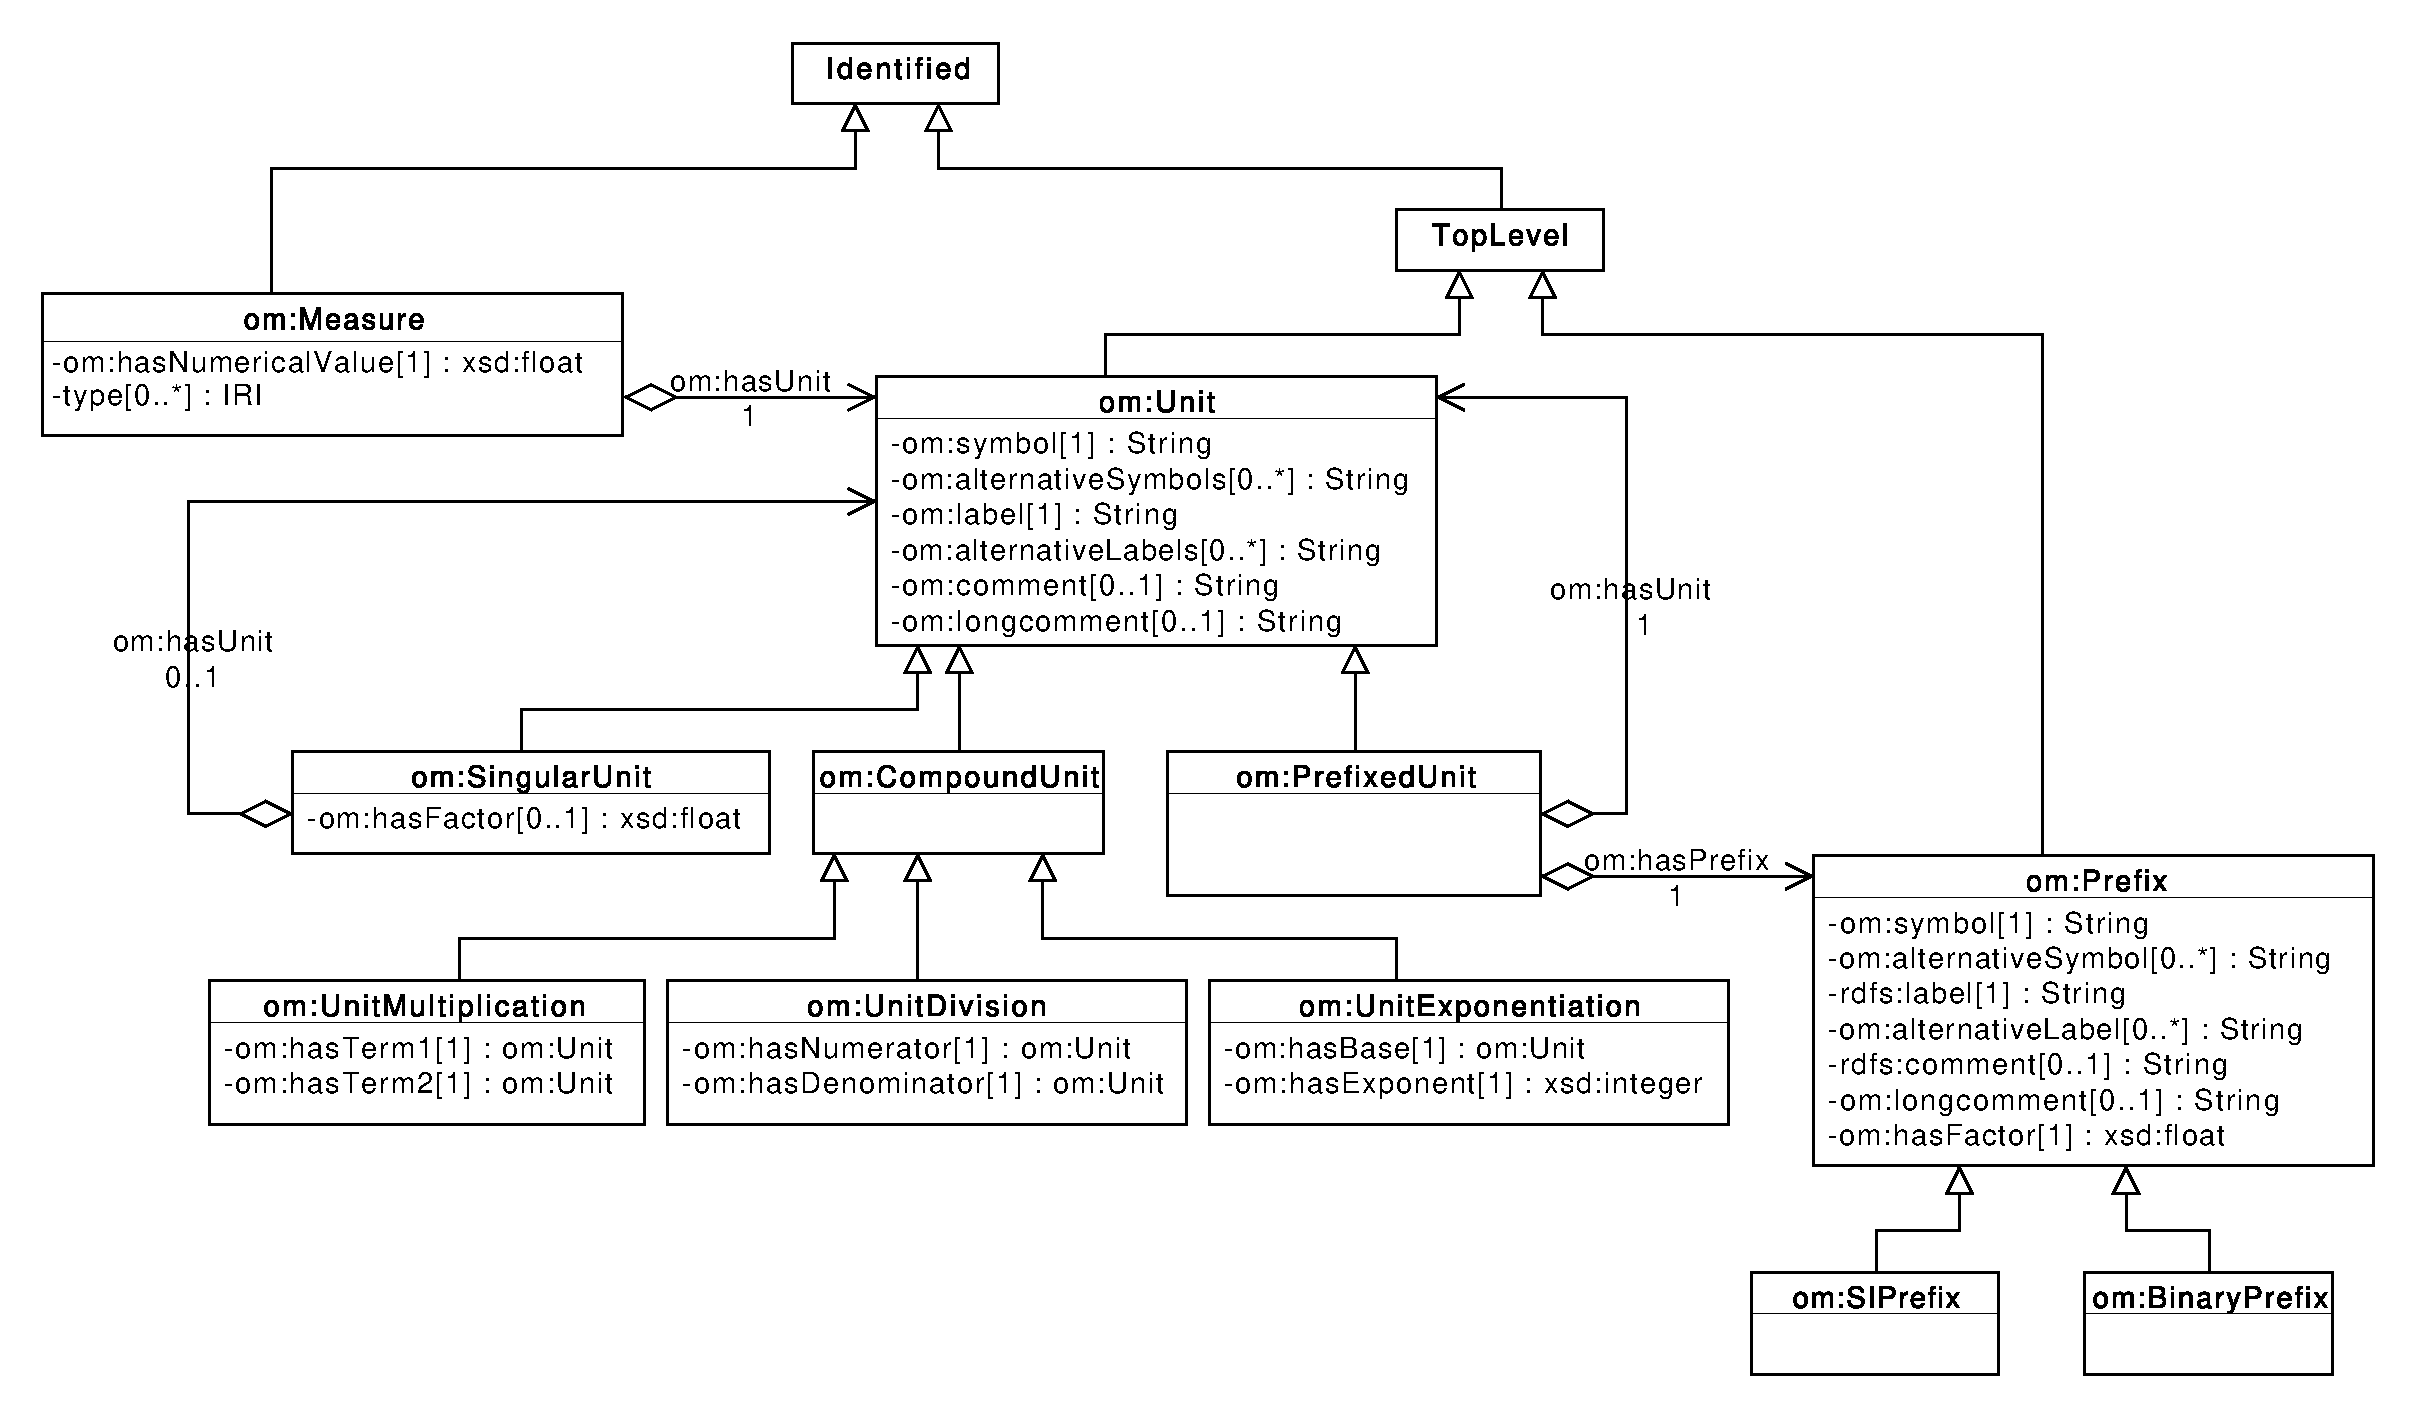
\includegraphics[width=\linewidth]{uml/om}
\caption[]{OM classes adopted by SBOL and their subclass relationships to \sbol{Identified} and \sbol{TopLevel}}
\label{uml:om}
\end{center}
\end{figure}

SBOL-compliant tools are allowed to read, write, and modify data belonging to OM classes other than those described here, but this specification does not provide any guidance for the interpretation or use of these data in the context of SBOL.
}


\twothreezero{
\subsubsection{Measure}
\label{sec:Measure}

The purpose of the \sbol{Measure} class is to link a numerical value to a \sbol{Unit}. 

\paragraph{The \sbolheading{hasNumericalValue} property}\label{sec:hasNumericalValue}
The \sbol{hasNumericalValue} property is REQUIRED and MUST contain a single xsd:float.

\paragraph{The \sbolheading{hasUnit} property}\label{sec:hasUnit:Measure}
The \sbolmult{hasUnit:Measure}{hasUnit} property is REQUIRED and MUST contain a URI reference to a \sbol{Unit}. The OM provides URIs for many existing instances of the \sbol{Unit} class for reference (for example, \url{http://www.ontology-of-units-of-measure.org/resource/om-2/gramPerLitre}).

\paragraph{The \sbolheading{types} property}\label{sec:types:Measure}
The \sbolmult{types:Measure}{types} property is OPTIONAL and MAY contain a set of URIs. It is RECOMMENDED that these URIs identify terms from the Systems Biology Ontology (SBO) (\url{http://www.ebi.ac.uk/sbo/main/}). This \sbolmult{types:Measure}{types} property is not specified in the OM and is added by SBOL to describe different types of parameters (for example, rate of reaction is identified by the SBO term \url{http://identifiers.org/biomodels.sbo/SBO:0000612}).

\paragraph{Serialization}
The serialization of a \sbol{Measure} MUST have the following form:
}

\lstsetsbol
\begin{lstlisting}
<prov:Measure rdf:about="...">
  ... [\emph{properties inherited from Identified}] ...
  [\emph{one}]  <om:hasNumericalValue>...</om:hasNumericalValue> [\emph{element}]
  [\emph{one}]  <om:hasUnit rdf:resource="..."/> [\emph{element}]
  [\emph{zero or more}]  <sbol:types rdf:resource="..."/> [\emph{element}]
</prov:Measure>
\end{lstlisting}

\twothreezero{
The example below shows the serialization of a \sbol{Measure} that represents the Michaelis constant for an enzymatic reaction.
}
\lstsetsbol
\begin{lstlisting}
<?xml version="1.0" ?>
<rdf:RDF xmlns:rdf="http://www.w3.org/1999/02/22-rdf-syntax-ns#" xmlns:dcterms="http://purl.org/dc/terms/" xmlns:om="http://www.ontology-of-units-of-measure.org/resource/om-2/" xmlns:xsd="http://www.w3.org/2001/XMLSchema#" xmlns:sbol="http://sbols.org/v2#">
  <sbol:Measure rdf:about="http://sbolstandard.org/example/ribonuclease_michaelis_constant/1">
    <sbol:persistentIdentity rdf:resource="http://sbolstandard.org/example/ribonuclease_michaelis_constant"/>
    <sbol:displayId>ribonuclease_michaelis_constant</sbol:displayId>
    <dcterms:title>Ribonuclease Michaelis Constant</dcterms:title>
    <om:hasNumericalValue>"7.9"^^xsd:float<om:hasNumericalValue/>
    <om:hasUnit rdf:resource="http://www.ontology-of-units-of-measure.org/resource/om-2/millimolair"/>
    <sbol:type rdf:resource="http://identifiers.org/biomodels.sbo/SBO:0000027"/>
  </sbol:Measure>
</rdf:RDF>
\end{lstlisting}
\label{ser:Measure}


\twothreezero{
\subsubsection{Unit}
\label{sec:Unit}

The purpose of the \sbol{Unit} class is to describe a particular unit of measure. 

\paragraph{The \sbolheading{symbol} property}\label{sec:symbol:Unit}
The \sbolmult{symbol:Unit}{symbol} property is REQUIRED and MUST contain a \sbol{String}. This \sbol{String} is commonly used to abbreviate the unit of measure's name. For example, the unit of measure named "gram per litre" is commonly abbreviated using the \sbol{String} "g/l".

\paragraph{The \sbolheading{alternativeSymbols} property}\label{sec:alternativeSymbols:Unit}
The \sbolmult{alternativeSymbols:Unit}{alternativeSymbols} property is OPTIONAL and MAY contain a set of \sbol{String}s. This property can be used to specify alternative abbreviations other than that specified using the \sbolmult{symbol:Unit}{symbol} property.

\paragraph{The \sbolheading{label} property}\label{sec:label:Unit}
The \sbolmult{label:Unit}{label} property is REQUIRED and MUST contain a \sbol{String}. This \sbol{String} is a common name for the unit of measure and SHOULD be identical to any \sbol{String} contained by the \sbol{name} property inherited from \sbol{Identified}.

\paragraph{The \sbolheading{alternativeLabels} property}\label{sec:alternativeLabels:Unit}
The \sbolmult{alternativeLabels:Unit}{alternativeLabels} property is OPTIONAL and MAY contain a set of \sbol{String}s. This property can be used to specify alternative common names other than that specified using the \sbolmult{label:Unit}{label} property.

\paragraph{The \sbolheading{comment} property}\label{sec:comment}
The \sbolmult{comment:Unit}{comment} property is OPTIONAL and MAY contain a \sbol{String}. This \sbol{String} is a description of the unit of measure and SHOULD be identical to any \sbol{String} contained by the \sbol{description} property inherited from \sbol{Identified}.

\paragraph{The \sbolheading{longcomment} property}\label{sec:longcomment}
The \sbolmult{longcomment:Unit}{longcomment} property is OPTIONAL and MAY contain a \sbol{String}. This \sbol{String} is a long description of the unit of measure and SHOULD be longer than any \sbol{String} contained by the \sbolmult{comment:Unit}{comment} property.
}

\twothreezero{
\subsubsection{SingularUnit}
\label{sec:SingularUnit}

The purpose of the \sbol{SingularUnit} class is to describe a unit of measure that is not explicitly represented as a multiplication, division, or exponentiation of two or more units, but could be equivalent to such a representation. For example, a joule is considered to be a \sbol{SingularUnit}, but it is equivalent to the multiplication of a newton and a meter.  

\paragraph{The \sbolheading{hasUnit} property}\label{sec:hasUnit:SingularUnit}
The \sbolmult{hasUnit:SingularUnit}{hasUnit} is OPTIONAL and MAY contain a URI. This URI MUST reference another \sbol{Unit}. The \sbolmult{hasUnit:SingularUnit}{hasUnit} propery can be used in conjunction with the \sbolmult{hasFactor:SingularUnit}{hasFactor} property to specify whether a \sbol{SingularUnit} is defined as another \sbol{Unit} multiplied by some factor. For example, an angstrom is defined as $10^{-10}$ meters.

\paragraph{The \sbolheading{hasFactor} property}\label{sec:hasFactor:SingularUnit}
The \sbolmult{hasFactor:SingularUnit}{hasFactor} property is OPTIONAL and MAY contain a xsd:float. If the \sbolmult{hasFactor:SingularUnit}{hasFactor} property of a \sbol{SingularUnit} is non-empty, then its \sbolmult{hasUnit:SingularUnit}{hasUnit} property SHOULD also be non-empty.

\paragraph{Serialization}
The serialization of a \sbol{SingularUnit} MUST have the following form:
}

\lstsetsbol
\begin{lstlisting}
<prov:SingularUnit rdf:about="...">
  ... [\emph{properties inherited from TopLevel}] ...
  [\emph{one}]  <om:symbol>...<om:symbol/> [\emph{element}]
  [\emph{zero or more}]  <om:alternativeSymbol>...<om:alternativeSymbol/> [\emph{element}]
  [\emph{one}]  <rdfs:label>...<rdfs:label/> [\emph{element}]
  [\emph{zero or more}]  <om:alternativeLabel>...<om:alternativeLabel/> [\emph{element}]
  [\emph{zero or one}]  <rdfs:comment>...<rdfs:comment/> [\emph{element}]
  [\emph{zero or one}]  <om:longcomment>...<om:longcomment/> [\emph{element}]
  [\emph{zero or one}]  <om:hasUnit rdf:resource="..."/> [\emph{element}]
  [\emph{zero or one}]  <om:hasFactor rdf:resource="..."/> [\emph{element}]
</prov:SingularUnit>
\end{lstlisting}

\twothreezero{
The example below shows the serialization of a \sbol{SingularUnit} that captures a genetic unit of length not present in the OM, the base pair (bp). One bp is equivalent to 3.4 angstroms.
}
\lstsetsbol
\begin{lstlisting}
<?xml version="1.0" ?>
<rdf:RDF xmlns:rdf="http://www.w3.org/1999/02/22-rdf-syntax-ns#" xmlns:dcterms="http://purl.org/dc/terms/" xmlns:om="http://www.ontology-of-units-of-measure.org/resource/om-2/" xmlns:xsd="http://www.w3.org/2001/XMLSchema#" xmlns:sbol="http://sbols.org/v2#">
  <sbol:SingularUnit rdf:about="http://sbolstandard.org/example/base_pair/1">
    <sbol:persistentIdentity rdf:resource="http://sbolstandard.org/example/base_pair"/>
    <sbol:displayId>base_pair</sbol:displayId>
    <dcterms:title>Base Pair</dcterms:title>
    <om:symbol>bp</om:symbol>
    <rdfs:label xml:lang="en">Base Pair</rdfs:label>
    <om:hasUnit rdf:resource="http://www.ontology-of-units-of-measure.org/resource/om-2/angstrom"/>
    <om:hasFactor rdf:datatype="&xsd;float">3.4</om:hasFactor>
  </sbol:SingularUnit>
</rdf:RDF>
\end{lstlisting}
\label{ser:Measure}


\twothreezero{
\subsubsection{CompoundUnit}
\label{sec:CompoundUnit}
}


\twothreezero{
\subsubsection{UnitMultiplication}
\label{sec:UnitMultiplication}

\paragraph{The \sbolheading{hasTerm1} property}\label{sec:hasTerm1}
The \sbol{hasTerm1} property

\paragraph{The \sbolheading{hasTerm2} property}\label{sec:hasTerm2}
The \sbol{hasTerm2} property

\paragraph{Serialization}
The serialization of a \sbol{UnitMultiplication} MUST have the following form:
}

\lstsetsbol
\begin{lstlisting}
<prov:UnitMultiplication rdf:about="...">
  ... [\emph{properties inherited from TopLevel}] ...
  [\emph{zero or more}]  <prov: rdf:resource="..."/> [\emph{element}] 
</prov:UnitMultiplication>
\end{lstlisting}


\twothreezero{
\subsubsection{UnitDivision}
\label{sec:UnitDivision}

\paragraph{The \sbolheading{hasNumerator} property}\label{sec:hasNumerator}
The \sbol{hasNumerator} property

\paragraph{The \sbolheading{hasDenominator} property}\label{sec:hasNumerator}
The \sbol{hasDenominator} property

\paragraph{Serialization}
The serialization of a \sbol{UnitDivision} MUST have the following form:
}

\lstsetsbol
\begin{lstlisting}
<prov:UnitDivision rdf:about="...">
  ... [\emph{properties inherited from TopLevel}] ...
  [\emph{zero or more}]  <prov: rdf:resource="..."/> [\emph{element}] 
</prov:UnitDivision>
\end{lstlisting}


\twothreezero{
\subsubsection{UnitExponentiation}
\label{sec:UnitExponentiation}

\paragraph{The \sbolheading{hasBase} property}\label{sec:hasBase}
The \sbol{hasBase} property

\paragraph{The \sbolheading{hasExponent} property}\label{sec:hasExponent}
The \sbol{hasExponent} property

\paragraph{Serialization}
The serialization of a \sbol{UnitExponentiation} MUST have the following form:
}

\lstsetsbol
\begin{lstlisting}
<prov:UnitExponentiation rdf:about="...">
  ... [\emph{properties inherited from TopLevel}] ...
  [\emph{zero or more}]  <prov: rdf:resource="..."/> [\emph{element}] 
</prov:UnitExponentiation>
\end{lstlisting}


\twothreezero{
\subsubsection{PrefixedUnit}
\label{sec:PrefixedUnit}

\paragraph{The \sbolheading{hasUnit} property}\label{sec:hasUnit:PrefixedUnit}
The \sbolmult{hasUnit:PrefixedUnit}{hasUnit} property

\paragraph{The \sbolheading{hasPrefix} property}\label{sec:hasPrefix}
The \sbol{hasPrefix} property

\paragraph{Serialization}
The serialization of a \sbol{PrefixedUnit} MUST have the following form:
}

\lstsetsbol
\begin{lstlisting}
<prov:PrefixedUnit rdf:about="...">
  ... [\emph{properties inherited from TopLevel}] ...
  [\emph{zero or more}]  <prov: rdf:resource="..."/> [\emph{element}] 
</prov:PrefixedUnit>
\end{lstlisting}


\twothreezero{
\subsubsection{Prefix}
\label{sec:Prefix}

\paragraph{The \sbolheading{symbol} property}\label{sec:symbol:Prefix}
The \sbolmult{symbol:Prefix}{symbol} property

\paragraph{The \sbolheading{hasFactor} property}\label{sec:hasFactor:Prefix}
The \sbolmult{hasFactor:Prefix}{hasFactor} property

\paragraph{The \sbolheading{alternativeSymbols} property}\label{sec:alternativeSymbols:Prefix}
The \sbolmult{alternativeSymbols:Prefix}{alternativeSymbols} property

\paragraph{The \sbolheading{alternativeLabels} property}\label{sec:alternativeLabels:Prefix}
The \sbolmult{alternativeLabels:Prefix}{alternativeLabels} property

\paragraph{The \sbolheading{longcomment} property}\label{sec:longcomment:Prefix}
The \sbolmult{longcomment:Prefix}{longcomment} property
}


\twothreezero{
\subsubsection{SIPrefix}
\label{sec:SIPrefix}

\paragraph{Serialization}
The serialization of a \sbol{SIPrefix} MUST have the following form:
}

\lstsetsbol
\begin{lstlisting}
<prov:SIPrefix rdf:about="...">
  ... [\emph{properties inherited from TopLevel}] ...
  [\emph{zero or more}]  <prov: rdf:resource="..."/> [\emph{element}] 
</prov:SIPrefix>
\end{lstlisting}


\twothreezero{
\subsubsection{BinaryPrefix}
\label{sec:BinaryPrefix}

\paragraph{Serialization}
The serialization of a \sbol{BinaryPrefix} MUST have the following form:
}

\lstsetsbol
\begin{lstlisting}
<prov:BinaryPrefix rdf:about="...">
  ... [\emph{properties inherited from TopLevel}] ...
  [\emph{zero or more}]  <prov: rdf:resource="..."/> [\emph{element}] 
</prov:BinaryPrefix>
\end{lstlisting}